\documentclass[times, utf8, diplomski]{fer}
\usepackage{booktabs}
\usepackage{amssymb}
\usepackage{amsmath}
\usepackage{tikz,}
\usepackage{subcaption}
\usepackage{tabularx,ragged2e,booktabs,caption}
\usepackage{color, colortbl}
\usepackage{array}% http://ctan.org/pkg/array
\usepackage{amsthm}
\usepackage{bm}
\usepackage[thinlines]{easytable}
\usepackage{float}


\captionsetup[table]{name=Tablica}

\theoremstyle{definition}
\newtheorem{definition}{Definicija}[section]

\begin{document}

% TODO: Navedite broj rada.
\thesisnumber{2018}

% TODO: Navedite naslov rada.
\title{Očitavanje rukom pisanih identifikacijskih brojeva temeljeno
na dubokim modelima}

% TODO: Navedite vaše ime i prezime.
\author{Tomislav Božurić}
\maketitle

% Ispis stranice s napomenom o umetanju izvornika rada. Uklonite naredbu \izvornik ako želite izbaciti tu stranicu.
\izvornik

% Dodavanje zahvale ili prazne stranice. Ako ne želite dodati zahvalu, naredbu ostavite radi prazne stranice.
\zahvala{Zahvalio bih se obitelji na neizmjernoj potpori tijekom mog studija, mentoru doc.dr.sc. Marku Čupiću na korisnim savjetima i ukazanoj pomoći te kolegama koji su utrošili vrijeme na popunjavanje baze rukom pisanih identifikatora.}

\tableofcontents
\listoffigures


\chapter{Uvod}
Očitavanjem rukom pisanih identifikacijskih (cijelih) brojeva bavili su se mnogi radovi od kraja 90-ih godina do danas. Tada je fokus bio na samoj klasifikaciji pojedinačnih brojeva, no u ovome radu zadatak uključuje lokalizaciju i klasifikaciju rukom napisanih identifikatora. Za razliku od skeniranog teksta (teksta napisanog na računalu) javlja se dodatan problem specifičnosti rukopisa pojedine osobe. Tako kod rješavanja problema moramo imati na umu da neke osobe brojeve pišu izduženo, neke nakošeno, neke sitnijim fontom dok druge većim. Tako možemo nastaviti nabrajati do u nedogled različite specifičnosti pojedinog rukopisa. Zbog toga je potrebno napraviti model koji će se moći nositi s navedenim problemima. Potrebno je izgraditi model koji će kvalitetno generalizirati, odnosno koji će imati veliku generalizacijsku moć, a neće biti pristran pojedinom rukopisu. Iz navedenog razloga bit će potrebno sakupiti dovoljno veliku bazu rukom pisanih identifikatora od više različitih osoba. 

U posljednjih nekoliko godina duboko učenje postaje sve popularnije. Jedan od glavnih razloga tome jest porast računalne moći, konkretno grafičkih procesnih jedinica \engl{Graphics processing unit} odnosno grafičkih kartica. Također, stvaranje velikih baza podataka omogućilo je robusnije  učenje takvih mreža za specifične zadatke. Zbog vrlo dobrih rezultata dubokih neuronskih mreža na sličnim klasifikacijskim problemima duboki modeli su se nametnuli kao logičan izbor u ovome radu.

Kroz ovaj rad pokazat će se sustav s grafičkim korisničkim sučeljem \engl{Graphical User Interface} koji problem očitavanja rukom pisanih identifikatora rješava kroz četiri faze koje su detaljno opisane u nastavku ovoga rada. Na samome početku ulazna slika se procesira odnosno obrađuje (obavlja se pretvorba u sive nijanse, odvajanje prednjeg plana od pozadine tj. binarizacija, dilatacija, stanjivanje, centriranje metodom centra mase i interpolacija). Takva slika se predaje algoritmu koji traži spojene konture na slici odnosno lokacije pojedinih brojeva koji se naposljetku klasificiraju. Sve to je omogućeno kroz intuitivno i jednostavno grafičko korisničko sučelje koje korisniku omogućava na vrlo efikasan način označavanje tako rukom napisanih brojeva.
\chapter{Pregled područja}
Znanstveni članci koji se bave klasifikacijom rukom pisanih znamenaka počinju davati rezultate vrijedne pažnje samim krajem 80-ih godina prošlog stoljeća. Tijekom razvoja sustava za klasificiranje rukom pisanih brojeva kroz povijest nastajale su razne baze podataka koje su korištene za ispitivanje kvalitete odnosno točnosti pojedinog sustava. Prva korištena baza podataka sastojala se od 1200 znamenki, poznatija kao "AT\&T". Baza se sastojala od 10 primjeraka svake znamenke od 12 različitih autora. Najčešće su znamenke od prvih 6 autora pripadale skupu za učenje, dok znamenke od preostalih 6 autora su pripadale skupu za testiranje odnosno validaciju. Zatim je nastala baza rukom pisanih poštanskih brojeva koja se sastojala od 7064 znamenke za treniranje i 2007 znamenaka za testiranje. Glavni nedostatak ovih baza jest vrlo mali skup za učenje i testiranje. U svrhu boljeg vrednovanja modela, nastala je baza znamenaka NIST. Glavni problem te baze je bio što su podaci iz skupa za učenje i skupa za testiranje bili iz potpuno različitih distribucija. Modifikacijom baze rukom pisanih brojeva NIST, nastala je danas najpoznatija baza imena MNIST, što dolazi od \textit{Modified} NIST. Originalno se testni skup NIST sastojao od 58527 slika znamenki napisanih od 500 različitih autora. Skup za ispitivanje NIST je podijeljen na primjerke od prvih 250 autora i dodan u novi skup za treniranje, dok su znamenke preostalih 250 autora dodane u skup za testiranje. Tako smo dobili otprilike 30000 znamenki u svakom od skupova. Novi skup za treniranje i testiranje nadopunjen je sa znamenkama iz prethodnog skupa za treniranje iz baze brojeva NIST. Najčešće se koristi 10000 znamenki za testiranje, dok se cijeli skup od 60000 znamenki koristi za treniranje.

\iffalse
Rad koji je davao \texttt{state-of-the-art} rezultate 1990. godine treniran jest nad 9298 znamenaka segmentiranih iz rukom pisanih poštanskih brojeva u Americi. Skup je bio nadopunjen s 3349 printanih znamenaka pisanih s 35 različitih fontova. Test za ispitivanje sadržavao jest 2007 rukom pisanih i 700 printanih znamenaka. Znamenke su bile ručno segmentirane odnosno odvojene jedna od druge. Cilj rada bio je pokazati kako je moguće da dovoljno velika back-propagation mreža može biti primijenjena na problem prepoznavanja slike bez velikog, kompleksnog preprocesiranja. Le Cun je još 1989 u svome radu pokazao kako arhitektura mreže značajno utječe na moć generalizacije same mreže. Smatrali su da dobra generalizacija se može dobiti dizajniranjem arhitekture mreže koja sadrži određenu količinu \textit{a priori} znanja o problemu. Mreža koju su koristili je bila višeslojna, sve konekcije u mreži su bile adaptivne, iako strogo ograničene, te je mreža trenirana koristeći algoritam back-propagation. Ulaz u mrežu bila je $16$x$16$ normalizirana slika na dimenzije $28$x$28$ i izlaz se očekivano sastojao od 10 jedinica. Pretpostavkom kako bi potpuno povezana neuronska mreža imala previše parametara i kako bi njezino treniranje u ono vrijeme trajalo jako dugo vremena, u radu se pojavljuje ideja lokalnih, konvolucijskih mapi značajki koje mogu biti primijenjene u slijednim skrivenim slojevima za ekstrakciju značajki veće kompleksnosti i apstrakcije. Mreža korištena za klasifikaciju je proširenje mreža opisanih u Le Cun 1989 i Le Cun et al., 1990a. Mreža je imala 4 skrivena sloja; H1, H2, H3, H4. Slojevi H1 i H2 bili su ekstraktori značajki s dijeljenim težinama, dok su H2 i H4 bili slojevi za uprosječivanje/sažimanje \engl{averaging/subsampling}. Prvi sloj se sastojao od 4 neovisne 24x24 mape značajki. Drugi sloj je bio sloj za uprosječivanje i sastojao se od 4 mape 12x12, zatim je opet slijedio sloj s 12 mapi značajki dimenzija 8x8, zatim sloj za uprosječivanje od 4 mape dimenzija 4x4 te naposljetku 10 izlaznih jedinica. U konačnici, mreža je imala 4635 jedinica, 98442 konekcije i 2578 neovisnih parametara. Na cijelom skupu za testiranja srednja kvadratna pogreška bila je 0.024, te su se sve pogreške dogodile na rukom klasifikaciji rukom pisanih znamenki.
\fi

Vrlo zanimljiv članak [\cite{LeCun95comparisonof}] uspoređuje klasifikatore koji su korišteni u brojnim do tada objavljenim znanstvenim člancima i koji su davali zapažljive rezultate. U nastavku slijedi kratak opis klasifikatora koji su se koristili u svrhu rješavanja navedenog zadatka (više detalja dostupno u citiranom članku). Cilj odlomka jest vrlo sažeto prikazati kakve su razne pristupe ljudi pokušavali kako bi dobili što kvalitetnije rezultate. Detaljniji opis s referencama na konkretne radove može se pronaći u detaljnijoj verziji prethodnog članka [\cite{Lecun95learningalgorithms}].
\\
Prvi od klasifikatora koji se pojavljuje jest \textit{osnovni linearni klasifikator} \engl{Baseline Linear Classifier}. Kao ulaz u klasifikator korištene su znamenke dimenzija 20x20. Svaka vrijednost ulaznog slikovnog elementa \engl{pixel} je sudjelovala u težinskoj sumi za svaku izlaznu jedinicu. Mreža je imala 4010 parametara (dodatnih 10 parametara su vezani za pristranost \engl{bias}) i klasifikator je postigao grešku na MNIST ispitnome skupu od 8.4\%.
\begin{figure}[h]
\centering
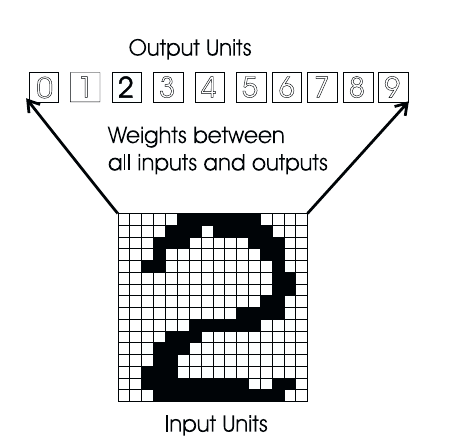
\includegraphics[scale=0.7]{linear_classifier.png}
\caption{Osnovni linearni klasifikator \\ (preuzeto iz \cite{Lecun95learningalgorithms})}
\end{figure}
\\
Slijedi klasifikator \textit{K najbližih susjeda} \engl{Baseline Nearest Neighbor Classifier} koji kao mjeru udaljenosti koristi Euklidsku udaljenost ulaznih slika. Njegova prednost jest što nema vrijeme učenja, niti je potrebno smišljati arhitekturu mreže. No, glavni mu je nedostatak što svih 60000 slika dimenzija 20x20 moraju biti u memoriji tijekom izvođenja kako bismo za neku ulaznu sliku pronašli kojoj slici odnosno znamenci je ta slika najbliža po Euklidskoj udaljenosti. Greška na MNIST testnome skupu za $k=3$ je bila 2.4\%. Inače, realističnija Euklidska udaljenost najbližeg susjeda bih se računala nad vektorom značajki, a ne direktno nad slikovnim elementima, no zbog usporedbe svih klasifikatora koji barataju direktno nad slikovnim elementima autor ovog rada odabrao je ovakav način usporedbe.
\\
\textit{Linearni klasifikator baziran na parovima} \engl{Pairwise Linear Classifier} je jednostavno poboljšanje prvog osnovnog modela jednostavnog linearnog klasifikatora. Ideja je bila da se svaki neuron jednoslojne mreže trenira da klasificira jednu klasu naspram ostalih. Odnosno u konkretnome radu, taj sloj je sadržavao 45 neurona labeliranih kao $0/1$, $0/2$,...,$0/9$,...$8/9$. Neuron $i/j$ je treniran da na izlazu daje $+1$ za uzorke klase $i$, a $-1$ za uzorke klase $j$. Pokazalo se da je rezultat nešto bolji nego s običnim linearnim klasifikatorom, greška je bila 7.6\% na spomenutome skupu.
\\
\textit{Metodom osnovnih komponenti i polinomijalnim klasifikatorom} \engl{Principal Component Analysis and Polynomial Classifier} uvedeno je predprocesiranje odnosno faza u kojoj se računa projekcija ulaznog uzorka na 40 glavnih komponenti koje predstavljaju ulazni uzorak. 40-dimenzionalni vektor je bio korišten kao ulaz u polinomijalni klasifikator drugog reda. Na testnome skupu postigao je grešku od 3.3\%.
\\
\textit{Mreža radijalnih baznih funkcija } \engl{Radial Basis Function Network-RBF} sastojala se od 1000 Gaussovih RBF neurona s 400 ulaza (slika dimenzija 20x20) te je drugi sloj bio jednostavan linearni klasifikator 1000$\rightarrow$10. Specifičnosti oko treniranja mogu se pronaći u navedenoj literaturi. Mreža je postigla grešku na testnome skupu od 3.6\%.
\\
\textit{Potpuno povezana višeslojna neuronska mreža} \engl{Fully Connected Multi-Layer Neural Network} s jednim skrivenim slojem trenirana je s različitim brojem neurona u skrivenom sloju. Najbolji postignuti rezultat je dobiven s mrežom $400-300-10$,  koja je približno imala 123300 težina. Dobivena greška na testnome skupu bila je 1.6\%. Tada je bilo misteriozno kako mreža s tako (tada) velikim brojem težina postiže tako malu grešku na ispitnome skupu. Pretpostavljali su da učenje gradijentnim spustom u višeslojnim mrežama ima efekt samo-regularizacije.
\\
Kako bi razriješili dilemu oko malih mreža koje nemaju dovoljno kapaciteta da nauče klasificirati skup za učenje i velikih mreža koje su preparametrizirane, dizajnirana je "specijalna" mreža imena \textit{LaNet1} za prepoznavanje dvo-dimenzionalnih oblika kao što su znamenke, koja eliminira irelevantne distorzije i varijabilnosti. Ta razmatranja dovode nas do danas vrlo popularnih \textbf{konvolucijskih mreža} [\cite{NIPS1989_293}], koje će biti detaljnije opisane u idućem poglavlju. Spomenimo kako dijeljenje težina u slojevima znatno smanjuje broj skrivenih parametara. Cijela mreža je formirana od više konvolucijskih slojeva, koji ekstrahiraju značajke rastuće kompleksnosti i apstrakcije. Mreža je učena back-propagation algoritmom, te su za razliku od prethodnih klasifikatora ulazne slike reducirane na veličinu 16x16 te su zatim centrirane na dimenzije 28x28 i proslijeđene ulaznom sloju. Mreža je imala samo 3000 slobodnih parametara, te je postigla rezultat od 1.7\% na MNIST ispitnome skupu. 1990. godine mreža ove arhitekture je bila \textit{state-of-the-art} mreža za klasifikaciju rukom pisanih brojeva.
\\
Eksperimentima nad \textit{LaNet 1} mrežom postalo je jasno da je potrebna konvolucijska mreža većeg kapaciteta da bi mogla kvalitetnije naučiti klasificirati uzorke iz skupa za učenje. \textit{LaNet 4} je "proširena" verzija LaNet1 mreže. Ulazni sloj je bio dimenzija 32x32,  a uzorci su centrirani u slike 20x20 metodom centra mase, koja je detaljnije opisana u poglavlju obrade slike. Mreža je sadržavala više mapi značajki, dodatan skriveni sloj i potpuno povezani sloj. Mreža je imala 260000 konekcija i 17000 slobodnih parametara. Postignuti rezultat na testnome skupu bio je 1.1\%.
\\
Mreža imena \textit{LaNet 5} imala je sličnu arhitekturu kao \textit{LaNet 4}, no imala je više mapi značajki, veći potpuno povezani sloj i drugačije je kodirala znamenke izlaznog sloja. Mreža je imala 340000 konekcija i 60000 slobodnih parametara, te je postigla grešku na ispitnome skupu od 0.9\%. Faza učenja uključivala je dodatan modul koji je uvodio distorziju na ulazne slike koristeći slučajno izabranu afinu transformaciju (pomak, skaliranje, rotacija i iskrivljavanje). Možemo primijetiti kako su povećanjem kapaciteta mreža dobiveni sve bolji i bolji rezultati, no treba imati na umu da mreža prevelikog kapaciteta može dovesti do prenaučenosti mreže.
\\
Poboljšana verzija \textit{LaNet 4} mreže imena \textit{Boosted LaNet 4} se sastojala od kombinacije 3 takve mreže. Prva mreža je učena klasičnim načinom, druga je učena nad  filtriranim uzorcima prve mreže tako da druga mreža vidi kombinaciju uzoraka. Konkretno, 50\% uzoraka koje je prva mreža dobro klasificirala i 50\% uzoraka na kojima je prva mreža pogriješila. Konačno, treća mreža je trenirana na novim uzorcima na kojima se nisu slagale prva i druga mreža. Kako je greška na skupu za učenje mreže \textit{LaNet 4} bila vrlo mala, bilo je potrebno povećati broj uzoraka za treniranje s nasumičnom distorzijom koristeći afine transformacije (kao kod \textit{LaNet 5} mreže) kako bi dobili dovoljan broj uzoraka za treniranje druge i treće mreže. Takve transformacije za povećavanje skupa za učenje odnosno testiranje popularne su i danas, te se često koriste kada nam je dostupan mali skup uzoraka za učenje i/ili validaciju. U konačnici, ova mreža je postigla grešku 0.7\% na ispitnome skupu. Očigledno jest da je vrijeme učenja ove mreže daleko veće nego kod \textit{LaNet 4} mreže. Pokazalo se da je trošak uvođenja tri mreže 1.75 puta veći nego kada smo koristili samo jednu mrežu. Ako je prva mreža s visokom pouzdanošću tvrdila da ulazni uzorak pripada nekoj od klasa brojeva, iduće dvije mreže nisu se niti razmatrale, pa se tako reducirao očekivani ukupni trošak.
\\
Memorijski baziran klasifikator imena \textit{Tangent Distance Classifier - TDC} temelji se na metodi najbližih susjeda. Kao i kod klasičnog klasifikatora koji se temelji na metodi najbližih susjeda, testni uzorci se uspoređuju s labeliranim uzorcima iz skupa za učenje. Klasa uzorka u skupu za učenje koji je "najbliže" ispitnome uzorku inicira klasu testnog uzorka. Ključno pitanje se postavlja što znači "blizu" u kontekstu uzoraka sa znamenkama. U naivnome pristupu, klasifikator koji se temelji na najbližim susjedima koristi Euklidsku udaljenost kod koje neporavnatost između inače "identičnih" slika može dovesti do velike udaljenosti. Ovaj klasifikator koristi mjeru udaljenosti koja je otporna na male distorzije, uključujući varijacije u debljini konture, translaciju, rotaciju, skaliranje i slično. Na MNIST testnome skupu klasifikator je imao 1.1\% pogrešku.
\\
Klasifikator imena \textit{Optimal Margin Classifier - OMC} možemo poistovjetiti sa strojem s potpornim vektorima \engl{Support Vector Machine} [\cite{Boser92atraining}] s mekim marginama [\cite{Cortes:1995:SN:218919.218929}]. Osnovna ideja SVM-a jest konstrukcija hiperravnine kao decizijske plohe ali tako da je margina odvajanja između "pozitivne" i "negativne" skupine uzorka (za učenje) maksimalna. Takva hiperravnina za koju je margina odvajanja maksimalna se naziva optimalna hiperravnina, te odatle izvorni naziv klasifikatora. Rezultirajuća arhitektura SVM-a se može promatrati kao dvoslojna neuronska mreža u kojoj su težine neurona prvog sloja potporni vektori koji računaju skalarni produkt između ulaza i njihovih težina. Za razliku od ostalih klasifikatora koji su postigli visoke performanse na skupu za ispitivanje, OMC ne uključuje \textit{a priori} znanje o problemu. No, i dalje je bio mnogo sporiji i trebao je više memorije za razliku od konvolucijskih mreža. Na MNIST bazi brojeva ovaj klasifikator je postigao grešku od 1.1\%.
\\
\begin{figure}[h]
\centering
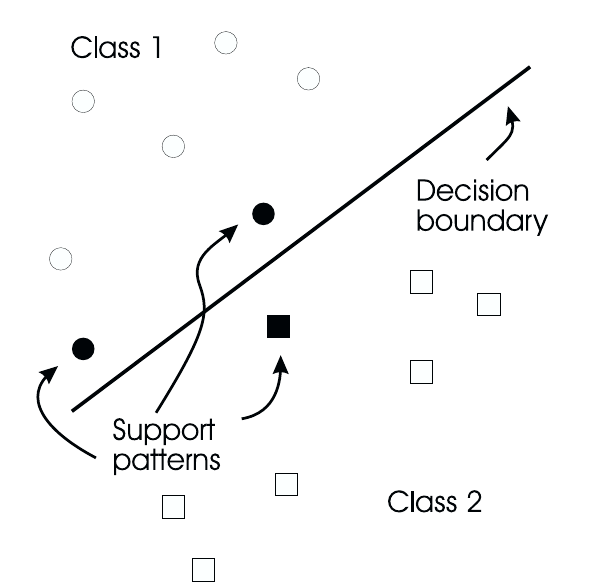
\includegraphics[scale=0.5]{omc_hyperplane.png}
\caption{Prikaz potpornih vektora i decizijske ravnine kod SVM-a  \\ (preuzeto iz \cite{Lecun95learningalgorithms})}
\end{figure}

Pokazalo se da, kada je dostupno mnogo uzoraka, mnoge metode mogu postići respektabilnu točnost. Iako treba primijetiti da neuronske mreže zahtijevaju relativno veliko vrijeme učenja, jednom kada se istreniraju zaključivanje provode mnogo brže i zahtijevaju puno manje memorije nego tehnike bazirane na memoriji. Trenutno najbolji rezultat na skupu uzoraka MNIST postignut jest konvolucijskom neuronskom mrežom i iznosi 0.23\% [\cite{6248110}]. Kasnijih godina isprobavani su razni pristupi s konvolucijskim mrežama, SVM-om, klasifikatorom temeljenom na najbližim susjedima itd. Mreže su postajale sve kompleksnije, imale su sve veći kapacitet i moć učenja te danas daju jako dobre rezultate, dok je vrijeme učenja neusporedivo manje. Zanimljiv članak [\cite{6490368}] koji govori o lokalizaciji registarskih oznaka koristeći tehnike procesiranja slike i genetske algoritme, na temelju analize povezanih komponenti pronalazi povezane objekte na samoj slici, a samim time i povezane alfanumeričke znakove unutar registarskih oznaka. Upravo metoda traženja povezanih komponenti je implementirana u ovome radu i davala je vrlo dobre rezultate. U članku [\cite{DL2018}] su iskoristili činjenicu da njihov klasifikator producira vjerojatnosnu distribuciju na izlazu. Zapazili su da kada ulaz sadrži znamenku, klasifikator producira distribuciju s malom entropijom i visokom pouzdanošću ispravne klase. S druge strane, kada ulaz ne sadrži znamenku, klasifikator producira gotovo uniformnu distribuciju. Tu činjenicu koriste za lokalizaciju znamenaka na slici. Sličnom idejom temeljenoj na entropiji i zbunjenosti modela izgrađeni klasifikator se koristi za detekciju potencijalno pogrešno označenih ili klasificiranih graničnih okvira. Više detalja nalazi se u poglavlju o izgrađenom sustavu.
\begin{figure}[h]
\centering
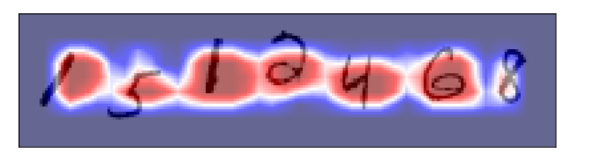
\includegraphics[scale=0.6]{localization_entropy.png}
\caption{Primjer lokalizacije na temelju vjerojatnosne distribucije na izlazu klasifikatora \\ (preuzeto iz \cite{DL2018})}
\end{figure}


\chapter{Umjetne neuronske mreže}
\section{Uvod}
Područje neuronskih mreža prvenstveno je inspirirano modeliranjem bioloških neuronskih sustava. Definiraju se i grade jednostavne procesne jedinice (umjetni neuroni) koje se potom povezuju u paralelne strukture različitih arhitektura poznate kao umjetne neuronske mreže \engl{Artificial Neural Networks}. Takav pristup poznat je još pod nazivom \textit{konektivistički pristup}, koji je prirodan za masovno raspodijeljeno i paralelno računanje. Neuronske mreže tijekom rada prolaze kroz dvije faze: \textit{fazu učenju} i \textit{fazu iskorištavanja}. Tijekom faze učenja neuronskoj mreži na ulazu se predočavaju uzorci iz skupa za učenje i uslijed toga dolazi do promjena težina, odnosno do promjena jakosti između veza neurona koji čine neuronsku mrežu. Samo učenje neuronske mreže može biti pojedinačno ili grupno. Poznate su i često korištene takozvane mini-grupe \engl{mini-batches}, koje se nalaze negdje između pojedinačnog i grupnog učenja. Kod \textit{pojedinačnog učenja} \engl{on-line learning} neuronska mreža uči nakon svakog predočenog uzorka, dok kod \textit{grupnog učenja} \engl{batch learning} neuronska mreža uči tek kada vidi čitav skup uzoraka za učenje. \newline
Razlikujemo i podjelu načina učenja neuronske mreže. Neuronska mreža može \textit{učiti s učiteljem} (nadzirano učenje) \engl{supervised learning}, \textit{učiti podržano} \engl{reinforcement learning} te učiti bez učitelja (nenadzirano) \engl{unsupervised learning} gdje želimo grupirati uzorke u određene grupe \engl{clustering}. U ovome radu koristi se nadzirano učenje, gdje se na ulaz konvolucijske mreže dovode ulazne slike i željeni izlazi. Mreža na ulaz dobiva uzorke oblika \textit{\{(slika znamenke, željeni izlaz), ..., (slika znamenke, željeni izlaz)\}}, koji se "dovode" u mini-grupama što je detaljno opisano u poglavlju implementacije.
\section{Biološki i umjetni model neurona}
Osnovna procesna jedinica mozga jest neuron. U ljudskom živčanom sustavu možemo naći približno $86$ milijardi neurona koji su povezani s približno $10^{14}$ - $10^{15}$ sinapsi \engl{synapses}. Svaki od neurona prima ulazne signale preko dendrita \engl{dendrites} i generira izlazni signal duž aksona \engl{axon}. Akson se na kraju grana i povezuje preko sinapsa s dendritima drugih neurona. U umjetnome modelu signali koji putuju duž aksona $x_0$ se množe s dendritima drugog neurona ($x_0w_0$) na temelju jačine sinapse $w_0$. Osnovna ideja jest da jakost sinapse se može mijenjati odnosno učiti tijekom vremena i tako možemo kontrolirati utjecaj same veze. Povećanjem težine dajemo vezi veći utjecaj, analogno vrijedi za smanjenje težine $w$. U osnovnom modelu dendriti prenose signale do tijela stanice gdje se svi signali zbrajaju. Dakle, tijelo stanice umjetnog neurona modelira integriranje svih primljenih pobuda u jedan zajednički potencijal stanice.
\begin{figure}[h]
\centering
\begin{subfigure}{.5\textwidth}
\centering
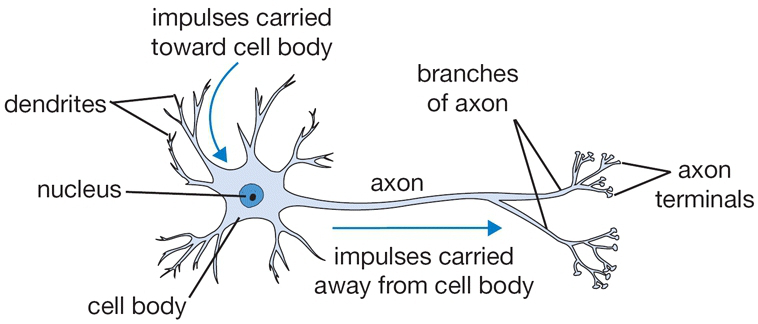
\includegraphics[width=\linewidth]{neuron.png}
\caption{Biološki neuron}
\label{fig:sub1}
\end{subfigure}%
\begin{subfigure}{.5\textwidth}
\centering
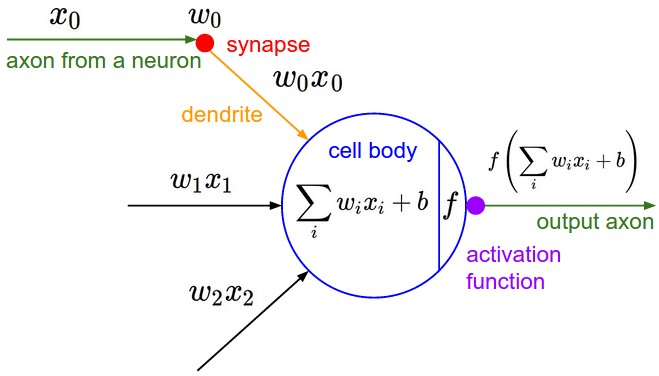
\includegraphics[width=\linewidth]{neuron_model.jpeg}
\caption{Umjetni neuron}
\label{fig:umjetni}
\end{subfigure}
\caption{Usporedba modela biološkog i umjetnog neurona \\ (preuzeto iz \cite{karpathy})}
\label{fig:usporedba_modela}
\end{figure}

Akson umjetnog neurona na slici \ref{fig:umjetni} prikazan je kao prijenosna funkcija \engl{transfer function} koja modelira prolaz signala kroz akson biološkog neurona. Općeniti izlaz umjetnog neurona možemo prikazati kao:
\begin{equation}
output = f(\sum_{i=0}^{n}w_ix_i + b)
\end{equation}
Povijesno gledano, uobičajeni izbor aktivacijske funkcije je sigmoidalna funkcija $\sigma$ koja uzima vrijednost izlaza iz tijela stanice i skalira ga u rasponu od $0$ do $1$. Kroz povijest koristile su se mnoge prijenosne funkcije poput  navedene sigmoidalne funkcije, funkcije identiteta, funkcije skoka i funkcije tangens hiperbolni. Razvojem dubokog učenja, u posljednjih nekoliko godina sve više se koriste ispravljena linearna funkcija (ReLu) \engl{Rectified Linear Unit}, slabo-ispravljena linearna funkcija (Leaky ReLu) \engl{Leaky Rectified Linear Unit} i \textit{maxout} neuroni.

\begin{figure}
\begin{subfigure}[t]{.5\textwidth}
\centering
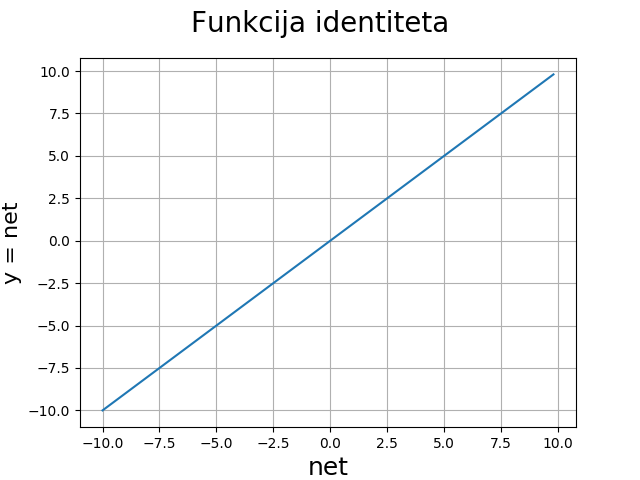
\includegraphics[width=\linewidth]{funkcija_identiteta.png}
\caption{Funkcija identiteta $f(net) = net$}
\end{subfigure}
\hfill
\begin{subfigure}[t]{.5\textwidth}
\centering
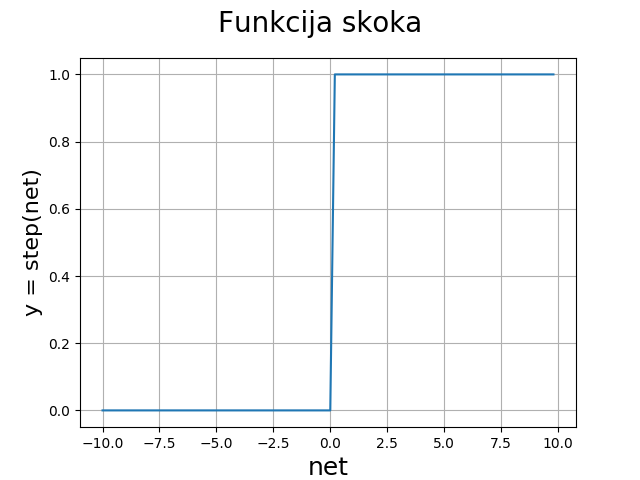
\includegraphics[width=\linewidth]{step_funkcija.png}
\caption{Funkcija skoka
$
f(net) = \begin{cases}
0, & net < 0\\
1, & net \geq 0\\
\end{cases}
$
}
\end{subfigure}
\medskip

\begin{subfigure}[t]{.5\textwidth}
\centering
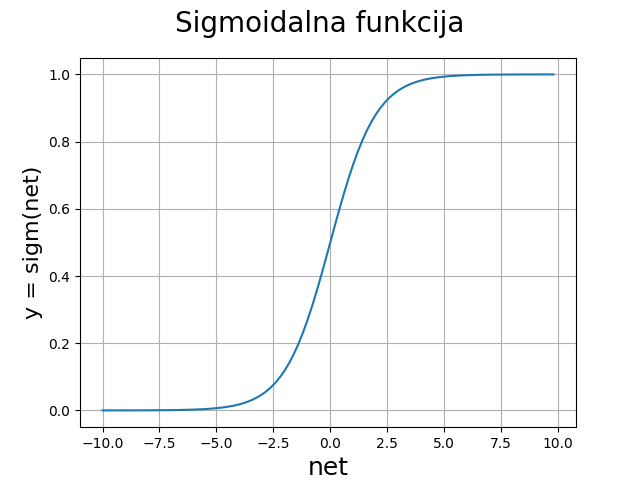
\includegraphics[width=\linewidth]{sigmoidalna_funkcija.png}
\caption{Sigmoidalna funkcija
$f(net) = \frac{1}{1 + e^{-net}}$
}
\end{subfigure}
\hfill
\begin{subfigure}[t]{.5\textwidth}
\centering
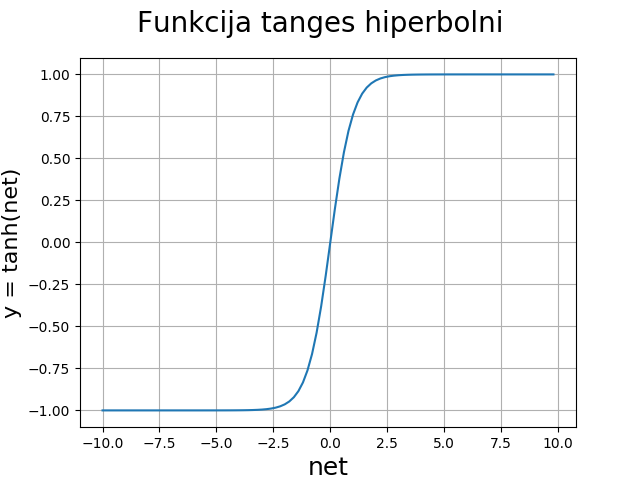
\includegraphics[width=\linewidth]{tanh_funkcija.png}
\caption{Funkcija tangens hiperbolni $f(net) = \tanh(net)$}
\end{subfigure}


\begin{subfigure}[t]{.5\textwidth}
\centering
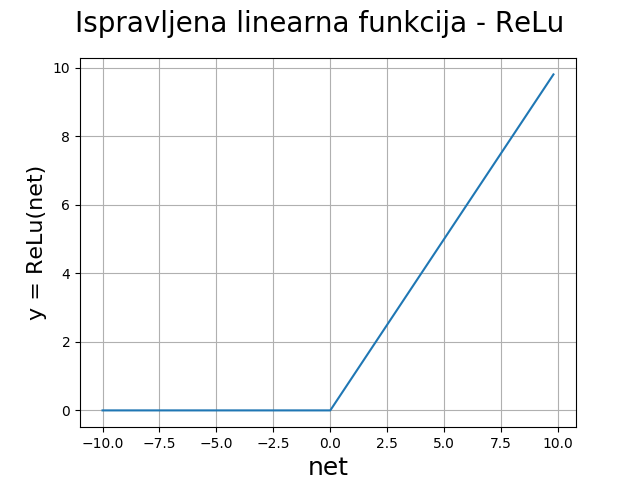
\includegraphics[width=\linewidth]{relu_funkcija.png}
\caption{ReLu funkcija
\centering
$
f(net) = \begin{cases}
0, & net < 0\\
net, & net \geq 0\\
\end{cases}
$
}
\end{subfigure}
\hfill
\begin{subfigure}[t]{.5\textwidth}
\centering
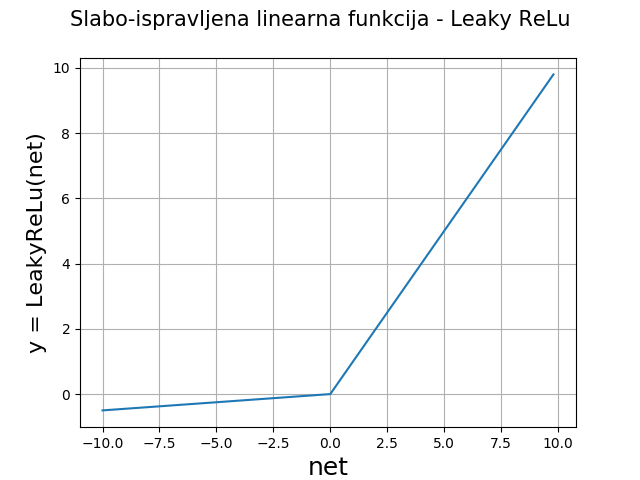
\includegraphics[width=\linewidth]{lrelu_funkcija.png}
\caption{Leaky ReLu funkcija, $a=0.1$
\centering
$
f(net) = \begin{cases}
a \cdot net, & net < 0\\
net, & net \geq 0\\
\end{cases}
$
}
\end{subfigure}
\caption{Prikaz najpoznatijih aktivacijskih funkcija}
\label{fig:activation_functions}
\end{figure}

Svaka od navedenih funkcija ima određenih prednosti i mana prilikom učenja mreža što i potiče istraživanje prikladnih aktivacijskih funkcija. Na slici \ref{fig:activation_functions} $net$ označava izlazni signal iz tijela stanice prije djelovanja aktivacijske funkcije.

\iffalse
\begin{table}[htbp]
\centering
\begin{tabular}{|>{\columncolor[gray]{0.6}}l|p{0.7\linewidth}| p{0.35\linewidth}|}
\hline
\multicolumn{1}{|c|}{\textit{\textbf{Cilj}}} & \multicolumn{1}{c|}{\textit{\textbf{Vrijednost}}} & \multicolumn{1}{c|}{\textit{\textbf{Težinski faktor}}} \tabularnewline \hline
$f_1$ & broj parova susjednih korištenih traka koje se razlikuju u parkiranoj seriji vozila & $\frac{1}{p_1}$ = broj korištenih traka $-1$ \\ \hline
$f_2$ & broj korištenih traka & $\frac{1}{p_2}$ = ukupni broj traka \\ \hline
$f_3$ & suma neiskorištenog kapaciteta na korištenim trakama & $\frac{1}{p_3}$ = ukupni kapacitet svih traka - ukupna duljina svih vozila \\ \hline
$g_1$ & broj parova susjednih vozila u traci s istim tipom rasporeda & $\frac{1}{r_1}$ = ukupni broj vozila u svim trakama - broj korištenih traka \\ \hline
$g_2$ & broj susjednih korištenih traka za koje vrijedi da zadnje vozilo u traci ima raspored istog tipa kao prvo vozilo u sljedećoj traci & $\frac{1}{r_2}$ = broj korištenih traka $-1$ \\ \hline
$g_3$ & suma nagrada i penala za vremenski razmak između polazaka, za sva susjedna vozila, u svim trakama
\begin{equation}
n=
\begin{cases}
15, & \text{$10\leq vr \leq 20 $} \\
10, & \text{$ vr > 20 $} \\
4\cdot(10-vr), & \text{$ vr < 10 $} \\
\end{cases}
\end{equation}
& $\frac{1}{r_3}$ = 15 $\cdot$ broj evaluiranih parova (susjeda iz traka) \\ \hline
\end{tabular}
\caption{Opis komponenti funkcija}
\label{table:komponente}
\end{table}
\fi
\section{Arhitektura neuronskih mreža}
Neuronske mreže su modelirane kao kolekcije neurona koji su povezani u acikličkom grafu u slojevitoj arhitekturi. Drugim riječima, izlazi nekih neurona mogu postati ulazi za druge neurone. Ciklusi nisu dozvoljeni jer bi to impliciralo beskonačnu petlju u unaprijednom prolazu kroz mrežu. Za klasične neuronske mreže najčešće korišteni tip sloja jest potpuno povezani sloj \engl{fully-connected layer} u kojem neuroni između dva susjedna sloja su potpuno po parovima povezani. Skup potpuno povezanih slojeva čini potpuno povezanu neuronsku mrežu \engl{fully-connected neural network}. Na slici možemo vidjeti potpuno povezanu neuronsku mrežu s 3 ulaza, dva skrivena sloja pri čemu u svakom od skrivenih slojeva imamo 4 neurona te jednim izlaznim neuronom. Mreža ima [3 x 4] + [4 x 4] + [4 x 1] = 32 težine i 4 + 4 + 1 = 9 pristranosti \engl{bias}.
\begin{figure}[h]
\centering
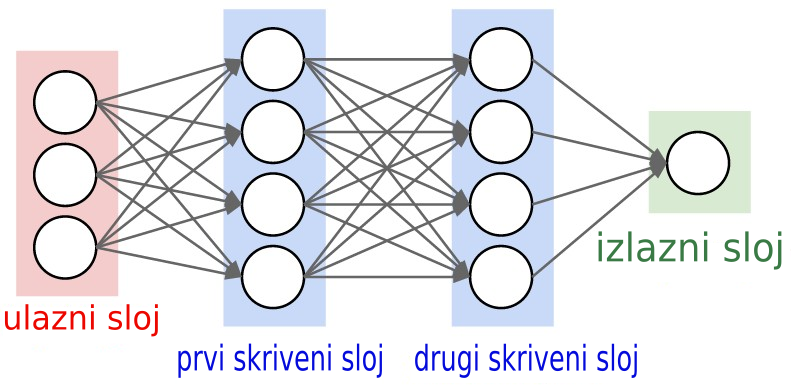
\includegraphics[scale=0.5]{neural_net2.png}
\caption{Potpuno povezana neuronska mreža s dva skrivena sloja}
\end{figure}


\chapter{Konvolucijske neuronske mreže}
\section{Uvod}
Konvolucijske neuronske mreže slične su običnim neuronskim mrežama, također se sastoje od neurona koji imaju težine i pristranosti koje se mogu učiti. Za razliku od običnih neuronskih mreža konvolucijske neuronske mreže čine eksplicitnu pretpostavku da su na ulazu slike, što nam omogućuje da kodiramo određene značajke u arhitekturu same mreže, odnosno ograničavaju arhitekturu na mnogo smisleniji način. Te pretpostavke nam omogućuju znatno smanjenje količine parametara same mreže, a samim time i veću vremensku efikasnost postupka učenja. Konkretno, za razliku od neuronskih mreža, konvolucijske neuronske mreže imaju neurone raspoređene u tri prostorne dimenzije: širinu, visinu i dubinu (gdje se dubina u ovome kontekstu ne odnosi na ukupan broj slojeva mreže nego na treću dimenziju tenzora). Sami duboki modeli imaju šansu naučiti značajke koji reagiraju na određene dijelove nama interesantnog objekta.

\begin{figure}[h]
\centering
\begin{subfigure}{.5\textwidth}
\centering
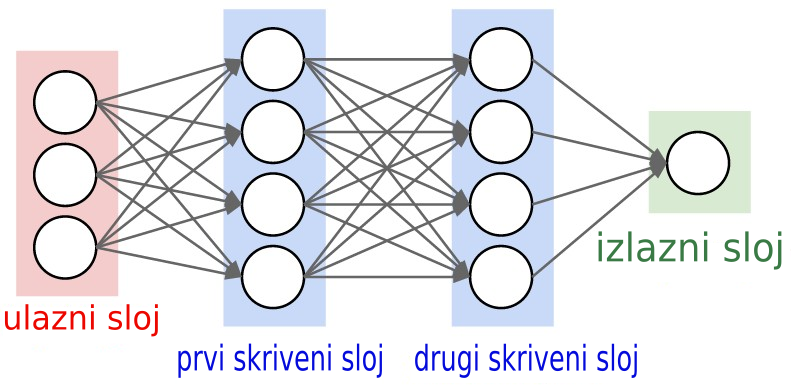
\includegraphics[width=\linewidth]{neural_net2.png}
\caption{Potpuno povezana neuronska mreža}
\label{fig:sub1}
\end{subfigure}%
\begin{subfigure}{.5\textwidth}
\centering
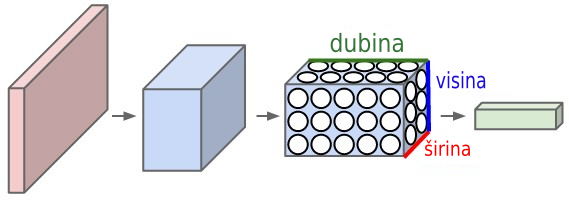
\includegraphics[width=\linewidth]{cnn.png}
\caption{Konvolucijska neuronska mreža}
\label{fig:sub2}
\end{subfigure}
\caption{Usporedba obične i konvolucijske neuronske mreže}
\label{fig:test}
\end{figure}

Specifičnost konvolucijskih modela jest da su transformacije lokalne, odnosno izlaz ovisi o lokalnom susjedstvu slikovnog elementa ulaza. Propuštanjem ulazne slike kroz konvolucijski model vršimo transformaciju trodimenzionalnih (3D) tenzora. U nastavku slijedi pregled klasične strukture takvih modela te kratak opis pojedinih slojeva koji su tipični kod konvolucijskih modela.
\begin{figure}
\centering
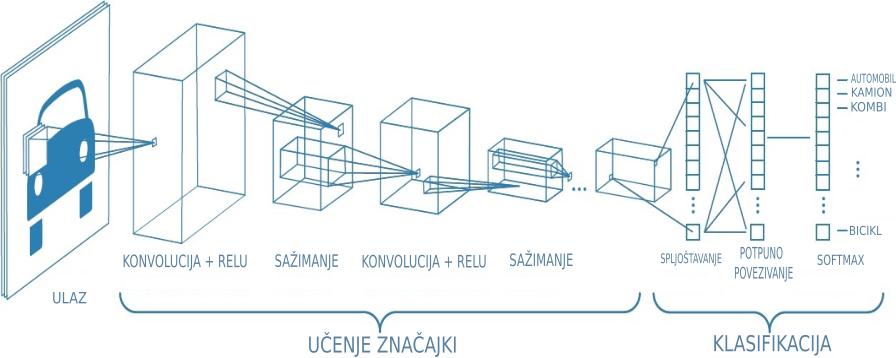
\includegraphics[scale=0.3]{architecture.png}
\caption{Primjer arhitekture konvolucijskog modela}
\end{figure}
\newpage Prvi od slojeva je konvolucijski sloj koji ekstrahira značajke iz ulazne slike. U najopćenitijem obliku, konvolucija jest operacija nad dvije funkcije s realnim domenama, koja daje modificiranu verziju jedne od dviju ulaznih (originalnih) funkcija.

\theoremstyle{definition}
\begin{definition}
Neka su $x(t)$ i $h(t)$ vremenski diskretne funkcije. \textbf{Konvolucija} funkcija $x$ i $h$ je definirana kao:
\begin{equation}
y(t) = \sum_{\tau=-\infty}^{\infty}x(\tau)h(t-\tau),
\end{equation}
te je kratko označavamo s $x(t) * h(t)$.
\end{definition}

\begin{figure}[h]
\centering
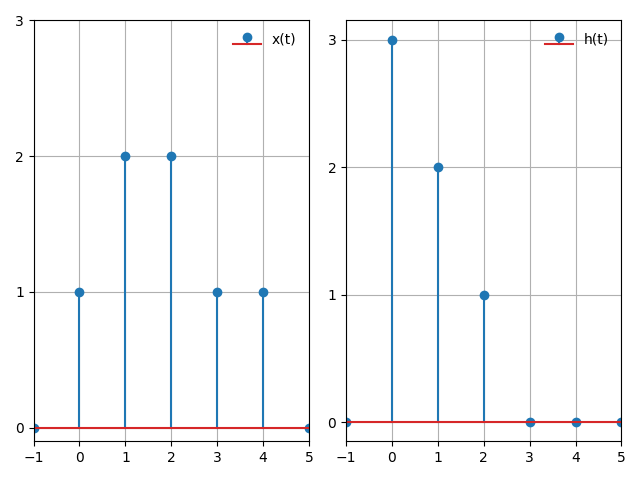
\includegraphics[scale=0.5]{convolution_discrete.png}
\caption{Ulazni diskretni signali $x(t)$ i $h(t)$}
\end{figure}



\begin{figure}[h]
\centering
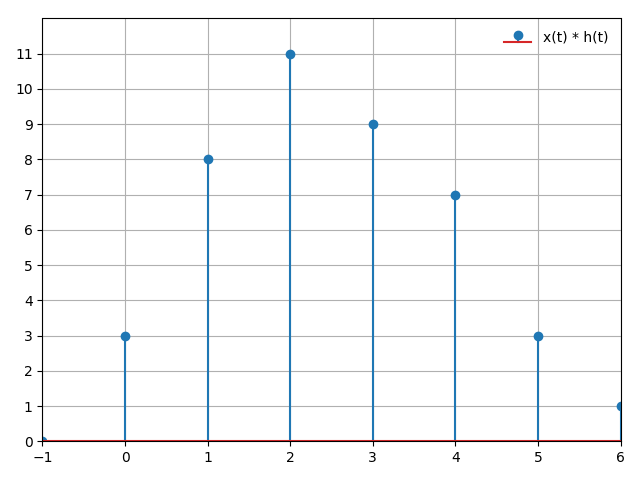
\includegraphics[scale=0.5]{convolution_result.png}
\caption{Rezultat konvolucije $x(t) * h(t)$}
\end{figure}


\begin{definition}
Neka su $x(t)$ i $h(t)$ vremenski neprekidne funkcije. \textbf{Konvolucija} funkcija $x$ i $h$ je definirana kao:
\begin{equation}
y(t) = \int_{\tau=-\infty}^{\infty}x(\tau)h(t-\tau)d\tau,
\end{equation}
te je kratko označavamo s $x(t) * h(t)$.
\end{definition}


\section{Konvolucija nad višedimenzionalnim signalima}
Očito jest da crno-bijelu fotografiju (monokromatsku fotografiju) - dimenzija N x M koja ima jedan ton možemo prikazati kao 2D signal njezinih prostornih koordinata.
\begin{equation}
x(n_H, n_W), 0\le n_H \le M-1, 0\le n_W \le N - 1,
\end{equation}
gdje su $n_H$ i $n_W$ diskretne prostorne koordinate na osima, a $x(n_H, n_W)$ predstavlja intenzitet slikovnog elementa na istoj diskretnoj prostornoj koordinati. Vrijednost koje poprima funkcija dvije varijable kreću se u intervalu $[0, 255]$. Slike koje se koriste kao ulaz u implementiranu konvolucijsku mrežu su binarne, odnosno poprimaju vrijednost intenziteta iz skupa \{$0, 255$\} odnosno \{0, 1\}.\newline
Promatramo li sliku s crvenim, zelenim i plavim kanalom (RGB) odnosno sliku dimenzija N x M x 3, signal možemo prikazati kao vektor 2D signala.

\begin{align*}
x(n_H, n_W) &= [x_R(n_H, n_W), x_G(n_H, n_W), x_B(n_H, n_W)] \\
&0\le n_H \le M-1, 0\le n_W \le N - 1,
\end{align*}
gdje $x_R$, $x_G$, $x_B$ označavaju intenzitet slikovnog elementa s obzirom na slijedno crveni, zeleni i plavi kanal.

\begin{definition}
Konvoluciju 2D slike $x(n_H, n_W)$, dimenzija N x M, s 2D filterom $h(n_H, n_W)$ definiramo kao:
\begin{equation}
y(n_H, n_W) = (x * h) (n_H, n_W) = \sum_{k = 0 }^{M-1}\sum_{l=0}^{N-1}x(k,l)h(n_h-k, n_w-l)
\end{equation}
gdje je $0\le n_H \le M-1, 0\le n_W \le N - 1$
\end{definition}
Konvolucija je komutativna pa možemo pisati:
\begin{equation}
y(n_H, n_W) = (x * h) (n_H, n_W) = \sum_{k = 0 }^{M-1}\sum_{l=0}^{N-1}x(n_h -k, n_w - l)h(k, l)
\end{equation}
U praksi komutativnost konvolucije nije važna, pa u primjenama koristimo kros-korelaciju \engl{cross-correlation} odnosno unakrsnu korelaciju:
\begin{equation}
y(n_H, n_W) = (x * h) (n_H, n_W) = \sum_{k = 0 }^{M-1}\sum_{l=0}^{N-1}x(n_h + k, n_w + l)h(k, l)
\end{equation}
Očigledno jest da u konkretnoj primjeni nam je svejedno na kojim će pozicijama algoritam naučiti vrijednosti jezgre. Ako koristimo klasičnu konvoluciju naučit ćemo iste vrijednosti kao i kada koristimo unakrsnu korelaciju, samo na obrnutim mjestima.

Prilikom razmatranja konvolucijskih neuronskih mreža, prvi argument konvolucije najčešće je ulazni uzorak a drugi argument je filter odnosno jezgra \engl{kernel}. Izlaz takve konvolucije nazivamo \textbf{mapa značajki} \engl{feature map}. Također, svaki element ulaznog uzorka i jezgre pohranjujemo zasebno, pa su vrijednosti funkcija u svim točkama nula osim u konačno mnogo točaka čije vrijednosti pohranjujemo. Konkretno, pretpostavljamo da je domena ulaza i jezgre konačan skup, tj. da su funkcije $x$ i $h$ izvan domene jednake 0. U primjenama su obično $x$ i $h$ višedimenzionalne funkcije $x(t), h(t) \in \mathbb{R}^d. $

Konvolucija čuva odnos između slikovnih elemenata učenjem značajki slike. U kontekstu konvolucijskih mreža, konvolucijom smatramo matematičku operaciju koja dobiva dva ulaza, matricu slike i filter odnosno jezgru \engl{kernel}. Konvolucijom slike s različitim filterima možemo vršiti operacije kao što su detekcija rubova, zamućivanje, izoštravanje i slično, te postoje poznati filteri koji se koriste u te svrhe.

\begin{figure}[h]
\centering
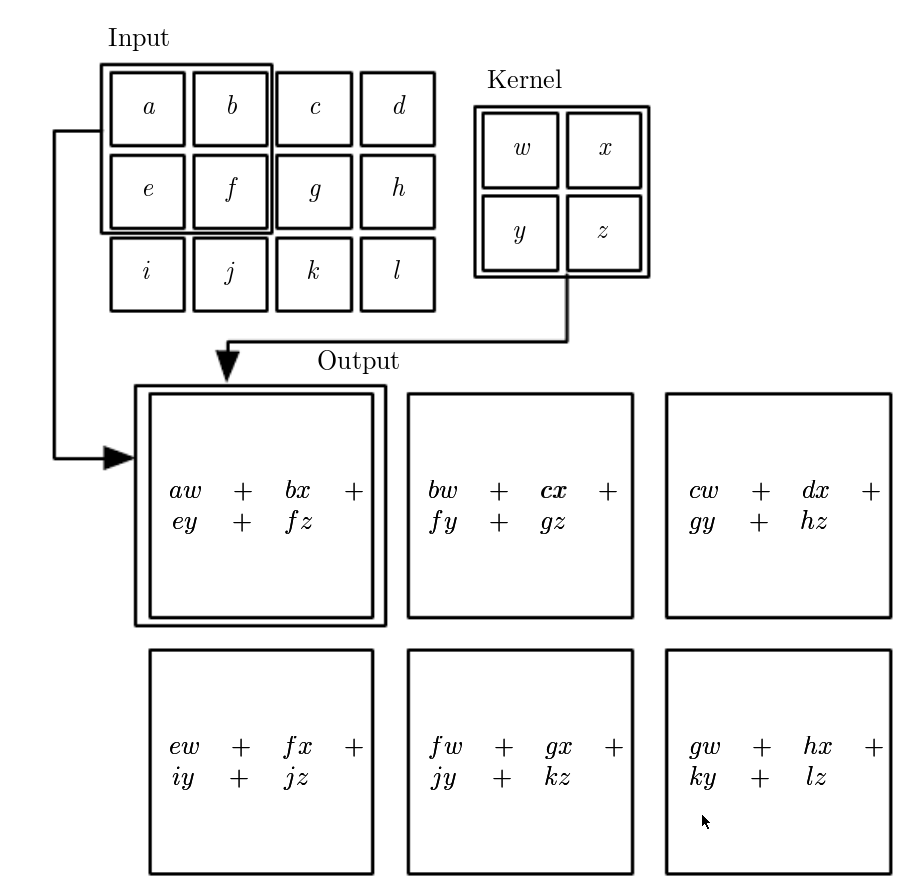
\includegraphics[scale=0.47]{convolution.png}
\caption{Konvolucija 2D ulaza i jezgre \\ (preuzeto iz \cite{Goodfellow-et-al-2016})}
\label{konvolucija_i_jezgra}
\end{figure}

//LOOK AT THIS
Iz gornje slike možemo primijetiti kako konvolucija modelira lokalne interakcije i dijeli parametre. Elementi  izlazne mape značajki (označimo je sa $M^l$) ovise o lokalnom susjedstvu elemenata ulazne mape značajki $M^{l-1}$ te se svi elementi mape značajki računaju pomoću istog skupa parametara \engl{shared weights}. Samo dijeljenje parametara ima više prednosti, osim što imamo znatno manji broj parametara dobivamo reprezentaciju ekvivarijantnu s obzirom na pomak.


\begin{figure}[h]
\begin{center}
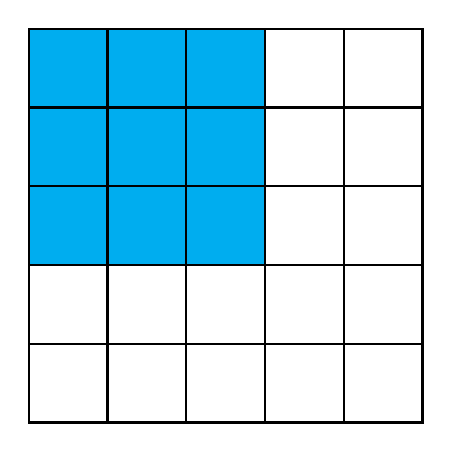
\begin{tikzpicture}
[%%%%%%%%%%%%%%%%%%%%%%%%%%%%%%
box/.style={rectangle,draw=black,thick, minimum size=1cm},
]%%%%%%%%%%%%%%%%%%%%%%%%%%%%%%

\foreach \x in {0,1,...,4}{
\foreach \y in {0,1,...,4}
\node[box] at (\x,\y){};
}
\node[box,fill=cyan ] at (0,2){};
\node[box,fill=cyan ] at (0,3){};
\node[box,fill=cyan] at (0,4){};

\node[box,fill=cyan ] at (1,2){};
\node[box,fill=cyan ] at (1,3){};
\node[box,fill=cyan ] at (1,4){};

\node[box,fill=cyan ] at (2,2){};
\node[box,fill=cyan ] at (2,3){};
\node[box,fill=cyan ] at (2,4){};
\end{tikzpicture}
\qquad
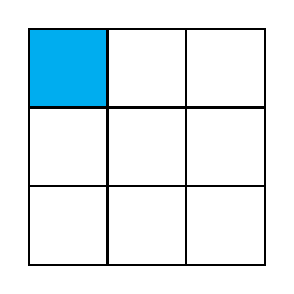
\begin{tikzpicture}
[%%%%%%%%%%%%%%%%%%%%%%%%%%%%%%
box/.style={rectangle,draw=black,thick, minimum size=1cm},
]%%%%%%%%%%%%%%%%%%%%%%%%%%%%%%

\foreach \x in {0,1,2}{
\foreach \y in {0,1,2}
\node[box] at (\x,\y){};
}
\node[box,fill=cyan] at (0,2){};
\end{tikzpicture}
\end{center}
\caption{Vizualizacija konvolucije filtera 3x3 na ulaznu sliku (lijevo) i dobivanje mape značajki (desno) }
\end{figure}
\newpage
\section{Lokalne interakcije i dijeljenje parametara}
Ranije je spomenuto da konvolucijom modeliramo samo lokalne interakcije. U ovom poglavlju daje se detaljniji osvrt na lokalne interakcije kod konvolucijskih mreža a zatim i na dijeljenje parametara.
Kod potpuno povezanog sloja svaki izlaz je povezan sa svim ulazima, dok kod konvolucije imamo povezanost samo s malim dijelom ulaza. Lokalna interakcija postiže se izborom filtera manjih dimenzija od samog ulaza. Tako dobivamo manje parametara (težina), manje potrebne memorije i manje potrebnih računskih operacija.

\begin{figure}[!htb]
\centering
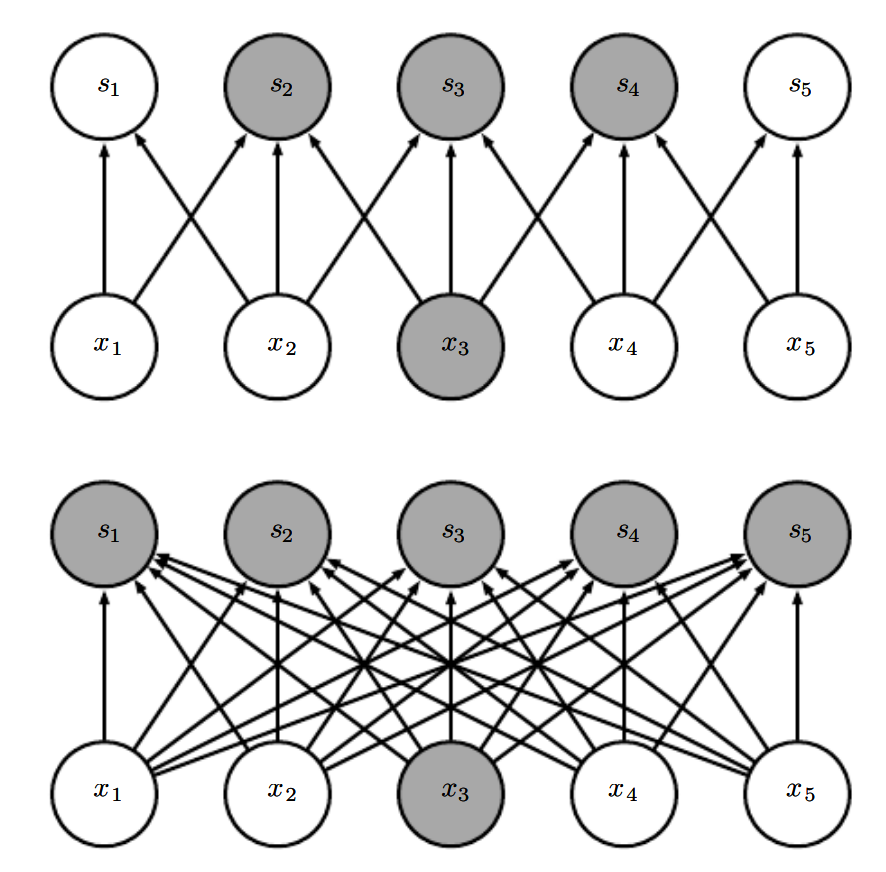
\includegraphics[scale=0.25]{lokalna_povezanost_odozdo.png}
\caption{Prikaz lokalne interakcije kod konvolucijskih mreža i interakcije kod potpuno povezane mreže gledano odozdo. Sivom bojom označen je ulazni neuron $x_3$ i izlazni neuroni $\bm{s}$ na koje utječe označeni ulazni neuron. \textit{Gore}: Kada $\bm{s}$ dobivamo konvolucijom s jezgrom širine 3, samo tri izlaza ovise o ulazu $\bm{x}$. \textit{Dolje}: Kada $\bm{s}$ promatramo u potpuno povezanom sloju, povezanost više nije rijetka, te su svi izlazi ovisni o ulaznom neuronu $x_3$ . \\ (preuzeto iz \cite{Goodfellow-et-al-2016})}
\end{figure}
\newpage

\begin{figure}[!htb]
\centering
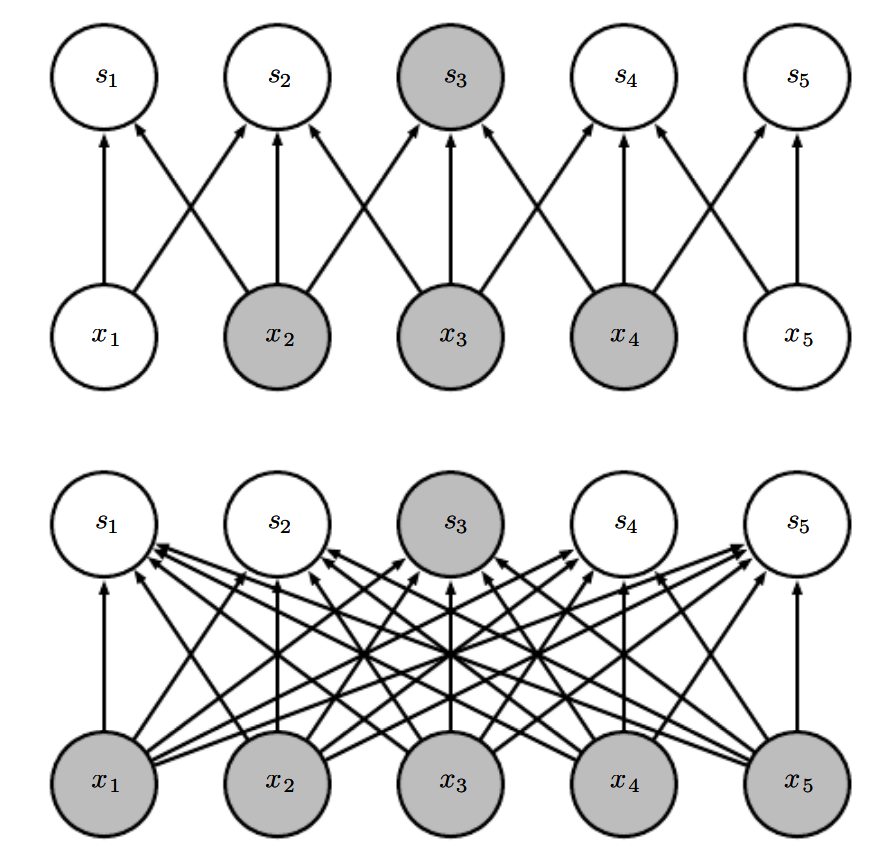
\includegraphics[scale=0.25]{lokalna_povetanost_odozgo.png}
\caption{Prikaz lokalne interakcije kod konvolucijskih mreža i interakcije kod potpuno povezane mreže gledano odozgo. Sivom bojom označen je jedan izlazni neuron $s_3$ i ulazni neuroni u $\bm{x}$ koji utječu na taj izlazni neuron. Ti neuroni su poznati pod nazivom \textbf{receptivno polje} \engl{receptive field} od $s_3$. \textit{Gore}: Kada je $\bm{s}$ dobiven konvolucijom s jezgrom širine 3, samo tri ulaza utječu na $s_3$. \textit{Dolje}: Kada je $\bm{s}$ dobiven matričnim množenjem, odnosno kada imamo potpuno povezani sloj, možemo primijetiti kako svi ulazni neuroni utječu na jedan neuron u idućem sloju, odnosno nemamo rijetku povezanost. \\ (preuzeto iz \cite{Goodfellow-et-al-2016}) }
\end{figure}
Receptivnim poljem značajke podrazumijevamo skup svih elemenata ulaznog sloja koje mogu utjecati na tu značajku, te je očito da ono raste s dubinom mreže.\newline

Za razliku od potpuno povezanih slojeva (mreža) glavna prednost jest da je potrebno naučiti manje parametara s istom količinom označenih podataka. Neka je $m$ broj ulaza a $n$ broj izlaza. Imamo li potpuno povezane slojeve odnosno matrično množenje zahtjeva $m$ x $n$ parametara te algoritam za svaki uzorak ima složenost $\mathcal{O}(m \cdot n)$. Ako ograničimo broj konekcija, pri čemu s $k$ označimo širinu jezgre ($k << m$), algoritam ima $k$ x $n$ parametara i složenost $\mathcal{O}(k \cdot n)$ (ovdje razmatramo samo lokalnost, a zanemarujemo dijeljenje parametara gdje se broj parametara još smanjuje) . Dakle imamo bržu evaluaciju $\mathcal{O}(m\cdot n)$ vs. $\mathcal{O}(k\cdot n)$.

Kod dijeljenja parametara umjesto učenja odvojenog skupa parametara za svaki od $n$ izlaza, svi izlazi dijele jedan te isti skup parametara. Svaka težina unutar filtera odnosno jezgre koristi se iznova na svakoj novoj poziciji ulazne aktivacijske mape \engl{feature map}. Dobivamo još manji model od samo $k$ parametara koji je teže prenaučiti. Samim time imamo bolju statističku efikasnost modela, dok je računska složenost evaluacija kao i kod modela koji samo ima lokalne interakcije $\mathcal{O}(k\cdot n)$. Dijeljenje parametara jednostavno možemo predočiti slikom \ref{konvolucija_i_jezgra}.

\section{Sloj sažimanja}
Funkcija sažimanja \engl{pooling function} mapira skup prostorno bliskih značajki na ulazu u jednu značajku na izlazu. Dakle, funkcije sažimanja reduciraju značajno broj parametara odnosno dimenzionalnost pojedine mape, no bitne (reprezentativne) informacije ostaju očuvane. Najčešće se računa statistički pokazatelj ulaznih značajki, primjerice prosječna ili maksimalna vrijednost. Ponekad se koristi i suma ulaznih značajki. Sažimanje nam je korisno kada tenzor prevodimo u simboličku kategoriju. Neki od tipova slojeva sažimanja koji se koriste su: \textit{sažimanje maksimalnom vrijednosti}, \textit{sažimanje srednjom vrijednosti}, \textit{sažimanje L2 normom}, \textit{sažimanje težinskim usrednjavanjem} i slično. Primjer sažimanja maksimalnom vrijednošću dan je u nastavku.
\begin{figure}[h]
\begin{center}
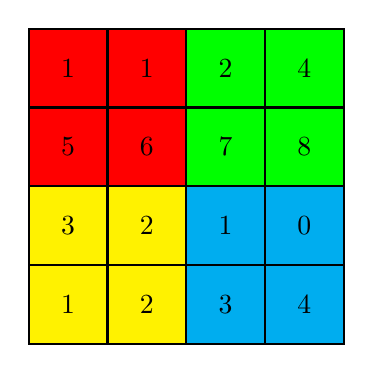
\begin{tikzpicture}
[%%%%%%%%%%%%%%%%%%%%%%%%%%%%%%
box/.style={rectangle,draw=black,thick, minimum size=1cm},
]%%%%%%%%%%%%%%%%%%%%%%%%%%%%%%

\foreach \x in {0,1,...,3}{
\foreach \y in {0,1,...,3}
\node[box] at (\x,\y){};
}
\node[box,fill=yellow] at (0,0){1};
\node[box,fill=yellow] at (0,1){3};
\node[box,fill=red] at (0,2){5};
\node[box,fill=red ] at (0,3){1};
\node[box,fill=yellow] at (1,0){2};
\node[box,fill=yellow] at (1,1){2};
\node[box,fill=red] at (1,2){6};
\node[box,fill=red ] at (1,3){1};
\node[box,fill=cyan] at (2,0){3};
\node[box,fill=cyan] at (2,1){1};
\node[box,fill=green] at (2,2){7};
\node[box,fill=green] at (2,3){2};
\node[box,fill=cyan] at (3,0){4};
\node[box,fill=cyan] at (3,1){0};
\node[box,fill=green] at (3,2){8};
\node[box,fill=green] at (3,3){4};
\end{tikzpicture}
\qquad
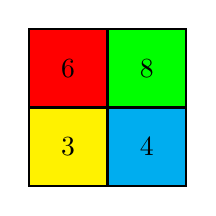
\begin{tikzpicture}
[%%%%%%%%%%%%%%%%%%%%%%%%%%%%%%
box/.style={rectangle,draw=black,thick, minimum size=1cm},
]%%%%%%%%%%%%%%%%%%%%%%%%%%%%%%
\foreach \x in {0,1}{
\foreach \y in {0,1}
\node[box] at (\x,\y){};
}
\node[box,fill=yellow] at (0,0){3};
\node[box,fill=red] at (0,1){6};
\node[box,fill=cyan] at (1,0){4};
\node[box,fill=green] at (1,1){8};
\end{tikzpicture}

\end{center}
\caption{Ulazna mapa značajki (lijevo) i rezultat djelovanja funkcije sažimanja (desno) temeljene na maksimalnoj vrijednosti koristeći jezgru 2x2 i korak \engl{stride} 2 }
\end{figure}

Sažimanje nam pomaže dobiti reprezentaciju koja je približno invarijantna na male translacije u ulazu. Invarijantnost na pomak znači da ako translatiramo malo ulaz, vrijednosti većine sažetih izlaza se ne mijenjaju. To svojstvo je vrlo korisno jer tako se fokusiramo na pitanje postoji li određena značajka, a ne gdje se točno nalazi. Primjerice, želimo li odrediti sadrži li slika lice, ne moramo znati striktno točnu lokaciju očiju, jedino nam je bitno da se jedno oko nalazi na lijevoj strani a drugo na desnoj strani. Povećanje invarijantnosti na pomak možemo matematički definirati kao $f(x)$ je invarijantna s obzirom na $g$ ako vrijedi $f(g(x)) =f(x)$. Veličina regije sažimanja regulira i dozu invarijantnosti, odnosno imamo li veće regije dobivamo veću invarijantnost na pomake. Sažimanje analogno možemo obaviti i preko različitih mapa značajki, tada mreža može naučiti invarijantnost i na druge transformacije kao što su rotacija i skaliranje.
Tipično prilikom primjene, sažimanje provodimo bez preklapanja ulaza. Svaku od (disjunktnih) regija sažimamo u jednu značajku nepromijenjene semantičke dimenzionalnosti. Samim time mapu značajki smanjujemo $k$ puta, gdje je $k$ veličina regije.

\begin{figure}[h]
\centering
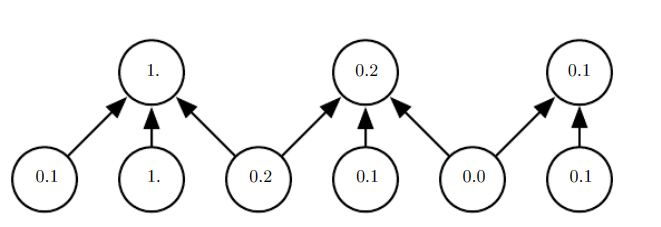
\includegraphics[scale=0.5]{pooling.png}
\caption{Prikaz sažimanja koristeći maksimalnu vrijednost \engl{max-pooling}. Širina kernela na slici je $3$ a korak je $2$. Tako smanjujemo reprezentaciju za faktor $2$, a samim time i reduciramo računski i statistički teret u idućem sloju. \\ (preuzeto iz \cite{Goodfellow-et-al-2016})}
\label{konvolucija}
\end{figure}

Uporabom sažimanja i konvolucija ugrađujemo pretpostavke u naš konvolucijski duboki model. Konvolucijom dobivamo interakcije koje su lokalne s obzirom na topologiju odnosno pretpostavljamo topologiju podataka i imamo predikciju kovarijantnu s pomakom. S druge strane sažimanjem dobivamo predikciju invarijantnu na male pomake. U praksi se pokazalo kako te pretpostavke ne dovode do podnaučenosti modela te da konvolucijski modeli bolje generaliziraju od potpuno povezanih modela iako u teoriji povećanje pristranosti i smanjenje varijance može dovesti do podnaučenosti.

\chapter{Obrada slike}
\section{Pretvorba slike u sive nijanse}
Prvi korišteni korak prilikom obrade slike jest pretvorba ulazne slike u sive nijanse. Većina digitalnih slika se sastoje od tri odvojena kanala: crveni kanal, zeleni kanal i plavi kanal. Stavljanjem tih slojeva jednog iznad drugog stvaramo sliku u boji. Različiti modeli boja imaju različite kanale, pa tako se možemo susresti sa situacijama kada su kanali boje, neke vrijednosti kao što su svjetlina ili saturacija (zasićenost) i slično. U ovome koraku primaran fokus je postavljen na prethodno spomenute RGB kanale pojedine slike.

Svaki algoritam pretvorbe slike u sive nijanse sastoji se od tri koraka.

\begin{enumerate}
\item Dohvaćanje crvene, zelene i plave vrijednosti slikovnog elementa
\item Korištenje matematičke funkcije za preslikavanje tih vrijednosti u specifičnu vrijednost koja predstavlja sivu nijansu
\item Zamjena crvene, zelene i plave vrijednosti s novo izračunatom vrijednošću sive nijanse
\end{enumerate}

\subsection{Uprosječivanje}
Metoda uprosječivanja je najjednostavnija metoda pretvorbe u sive nijanse i kako samo ime kaže vrijednost nijanse računa se sljedećim izrazom:
\begin{equation}
Gray = (Red + Green + Blue) / 3
\end{equation}
Iako je ova metoda najjednostavnija i najbrža, ne uzima u obzir pretpostavke o reprezentaciji sivih nijansi povezane s načinom kako ljudi percipiraju svjetlinu. Zbog toga je razvijeno još mnoštvo metoda koje se temelje na analizi ljudske percepcije boja i neke od tih metoda će biti opisane u nastavku.

\subsection{Poboljšanje temeljeno na ljudskoj percepciji boja}
Navedena metoda za razliku od prethodne u obzir uzima da ljudi "jače" percipiraju zelenu boju od crvene te crvenu "jače" od plave. To također ima smisla s gledišta evolucijske biologije, odnosno veliki dio prirode pojavljuje se u nijansama zelene boje, pa su tako ljudi boraveći u prirodnom okruženju razvili veću osjetljivost na zelenu boju. S obzirom na to da ljudi ne percipiraju sve boje jednako, možemo zaključiti da prethodna metoda uprosječivanja nijansi crvene, zelene i plave boje je neprecizna.
Umjesto tretiranja svih boja jednako, koristit ćemo pretvorbu gdje pojedinoj boji dajemo određen težinski faktor uzimajući u obzir ljudsko oko. Formula koju koriste i razni moćni alati za obradu slike je sljedeća:
\begin{equation}
Gray = Red \cdot 0.299 + Green \cdot 0.587 + Blue \cdot 0.114
\end{equation}

Gore navedena formula specificirana je standardom BT.601 koji se koristi u "modernim" digitalnim slikama i video formatima. Takav način pretvorbe boja daje sliku koja je dinamičnija.
Postoje neslaganja oko najboljeg načina pretvorbe boja, pa tako prema BT.709 standardu, formula za pretvorbu koja se ponekad u literaturi naziva \textit{Luma} izgleda ovako:
\begin{equation}
Gray = Red \cdot 0.2126 + Green \cdot 0.7152 + Blue \cdot 0.0722
\end{equation}
Upravo ta formula jest korištena u ovome radu za pretvorbu slika u sive nijanse.
Kao što je napomenuto, sami koeficijenti korišteni u težinskoj sumi, odnosno udio pojedine boje se temelji na brojnim analizama provedenih nad ljudskom shvaćanju boja.

\section{Binarizacija}
Binarne slike su one slike koje sadrže samo bijele i crne slikovne elemente. Odnosno postupkom binarizacije raspon boja od [0, 255] skaliramo na samo dvije vrijednosti (na 0 i 255 odnosno na 0 i 1). U ovome radu binarizacija je korištena za odvajanje prednjeg plana od pozadine, odnosno za odvajanje rukom pisanih identifikatora od bijele pozadine. Za binarizaciju slike u ovome radu korištena je Otsuova metoda koja na vrlo logičan način određuje prag binarizacije.
\subsection{Otsuova metoda binarizacija}
Otsuova metoda binarizacije pretpostavlja da ulazna slika čiji prag binarizacije želimo izračunati se sastoji od dvije klase slikovnih elemenata odnosno bi-modalnog histograma. Ako su zadovoljeni preduvjeti, računa se optimalni prag za separaciju tih dviju klasa tako da je varijanca unutar pojedine klase minimalna. Neke od glavnih prednosti ove metode su brzina, kvaliteta separacije klasa i jednostavnost implementacije.
\newline
\newline
Prvi korak prilikom binarizacije jest određivanja praga. Sam prag može biti određen ručno (primjerice postavimo li taj prag na 120, svi slikovni elementi čija siva komponenta jest iznad ili jednaka 120 postavimo na 255, dok sve ispod 120 postavimo na 0), no konstantni prag se nije pokazao najboljim u svim situacijama. Naravno, konstantni prag binarizacije je daleko najbrži, no kako ne daje uvijek najbolje rezultate taj prag je najbolje odrediti dinamički od slike do slike.
Metoda uključuje iteriranje kroz sve moguće vrijednosti praga i računa varijancu unutar razreda sa svake strane praga, odnosno za slikovne elemente koji pripadaju prednjem planu i slikovne elemente koji pripadaju pozadini. Cilj je pronaći vrijednost praga koja minimizira varijancu unutar razreda, definiranu kao težinsku sumu varijanci dviju klasa:

\begin{equation}
\sigma^2_{within}(t) = \omega_0(t)\sigma_0^2(t) + \omega_1(t)\sigma_1^2(t)
\end{equation}
Težine $\omega_0(t)$ i $\omega_1(t)$ su vjerojatnosti dviju klasa odvojenih pragom $t$, a $\sigma_0^2$ i $\sigma_1^2$ su varijance tih dviju klasa.

Vjerojatnosti klasa $\omega_{0,1}(t)$ se računaju iz $L$ vrijednosti stupaca histograma:

\begin{equation}
\begin{aligned}
\omega_0(t) = \sum_{i=0}^{t-1}p(i) \\
\omega_1(t) = \sum_{i=t}^{L-1}p(i)
\end{aligned}
\end{equation}
Postupak maksimizacije varijance između razreda iziskuje manji broj matematičkih operacija, pa samim time je i računalno efikasniji, a upravo je Otsu pokazao da je minimizacija varijance unutar razreda ekvivalentna maksimizaciji varijance između razreda:
\begin{equation}
\begin{aligned}
\sigma^2_{between}(t) = \sigma^2 - \sigma^2_{within}(t) = \omega_0(\mu_0 - \mu_T)^2 + \omega_1(\mu_1 - \mu_T)^2 = \omega_0(t)\omega_1(t)[\mu_0(t) - \mu_1(t)]^2
\end{aligned}
\end{equation}
Pri čemu su $\omega$ vjerojatnosti klasa, a $\mu$ očekivanja klasa.
U programskim implementacijama u standardnim bibliotekama se koristi maksimizacija varijance između razreda iz spomenutog razloga te je ona korištena i u ovome radu.


\begin{equation}
\begin{aligned}
\mu_0(t) = \frac{\sum_{i=0}^{t-1}ip(i)}{w_0(t)} \\
\mu_1(t) = \frac{\sum_{i=t}^{L-1}ip(i)}{w_1(t)} \\
\mu_T(t) = \sum_{i=0}^{L-1}ip(i)
\end{aligned}
\end{equation}
Navedene relacije mogu se vrlo lako provjeriti
\begin{equation}
\begin{aligned}
\omega_0\mu_0 + \omega_1\mu_1 = \mu_T \\
\omega_0 + \omega_1 = 1
\end{aligned}
\end{equation}

\textbf{Algoritam}

\begin{enumerate}
\item Izračunaj histogram i vjerojatnosti za svaku razinu intenziteta unutar histograma
\item Postavi inicijalne $\omega_i(0)$ i $\mu_i(0)$, za $i=0, 1$
\item Iteriraj kroz sve moguće vrijednosti pragova $t=1,...maksimalni\ intenzitet$
\subitem 1. Ažuriraj $\omega_i$ i $\mu_i$, za $i=0, 1$
\subitem 2. Izračunaj $\sigma^2_{between}(t)$
\item Željeni prag binarizacije odgovara pragu za koji je $\sigma^2_{between}$ poprimila najveću vrijednost
\end{enumerate}



\begin{figure}[h]
\centering
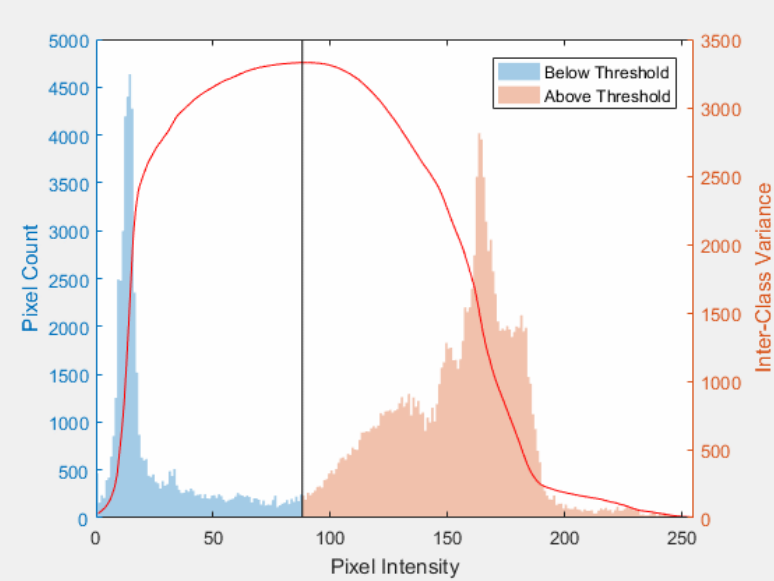
\includegraphics[scale=0.46]{otsu_method.png}
\caption{Prikaz određivanja praga binarizacije koristeći maksimizaciju varijance između razreda \\ (preuzeto iz \cite{ otsu:xxx})}
\end{figure}
Krivulja označena crvenom bojom predstavlja vrijednost varijance između razreda za pojedini prag binarizacije.
\section{Dilatacija}
Dilatacija je jedna od osnovnih operacija u matematičkoj morfologiji. Originalno je osmišljena za binarne slike, te se u ovome radu upravo nad takvim slikama i koristi. Operacija dilatacije koristi \textbf{strukturni element} za ispitivanje i proširenje oblika sadržanih u ulaznoj slici. Prilikom skeniranja ulazne slike na kojoj se nalaze rukom pisani brojevi možemo primijetiti određene nepravilnosti na samim konturama znamenaka. U svrhu podebljanja kontura znamenaka koristi se operacija dilatacije radi poboljšanja skupa za učenje, no i prilikom klasifikacije znamenaka sa slika iz skupa za ispitivanje. \newline
Dilatacija je u binarnoj morfologiji invarijantna na pomak i komutativna. Sama binarna slika u matematičkoj morfologiji se promatra kao podskup Euklidskog prostora ${\mathbb{R}^d}$ ili prostora cijelih brojeva $\mathbb{Z}^d$, gdje je $d$ dimenzija ulazne slike određene širine i visine. Neka je $A$ binarna slika definirana u Euklidskom prostoru ili u prostoru cijelih brojeva $E$ i neka je $B$ strukturni element podskup prostora ${\mathbb{R}^d}$. Tada je dilatacija binarne slike $A$ sa strukturnim elementom $B$ izražena izrazom:
\begin{equation}
A \oplus B = \bigcup_{b \in B} A_b
\end{equation}
Pri tome je $A_b$ translacija binarne slike $A$ s obzirom na $b$. Također zbog svojstva komutativnosti vrijedi:
\begin{equation}
A \oplus B = B \oplus A = \bigcup_{a \in A} B_a
\end{equation}
Korišteni strukturni element u ovome radu prikazan je u nastavku:
\[
b=
\begin{bmatrix}
1 & 1 & 1 \\
1 & 1 & 1 \\
1 & 1 & 1 \\
\end{bmatrix}
\]
\subsection{Primjer}
Neka je binarna slika definirana matricom:
\[
A=
\begin{bmatrix}
0 & 0 & 0 & 0 & 0 \\
0 & 0 & 1 & 0 & 0 \\
0 & 1 & 1 & 1 & 0 \\
0 & 0 & 1 & 0 & 0 \\
0 & 0 & 0 & 0 & 0 \\

\end{bmatrix}
\]

Neka je strukturni element:
\[
b=
\begin{bmatrix}
1 & 1\\
1 & 1\\
\end{bmatrix}
\]
Rezultat dilatacije binarne slike $A$ koristeći strukturni element $b$:

\[
C=
\begin{bmatrix}
0 & 1 & 1 & 1 & 0 \\
1 & 1 & \textbf{1} & 1 & 1 \\
1 & \textbf{1} & \textbf{1} & \textbf{1} & 1 \\
1 & 1 & \textbf{1} & 1 & 1 \\
0 & 1 & 1 & 1 & 0 \\

\end{bmatrix}
\]

Rezultat dobivamo tako da za svaki slikovni element u $A$ čija je vrijednost $1$, postavimo $b$ te "širimo" slikovne elemente u originalnoj slici s obzirom na strukturni element $b$. U radu se pokazalo kako je operacija dilatacije vrlo bitna za kvalitetu dobivenih klasifikacija mreže i pronalazak graničnih okvira oko samih znamenaka.

\section{Stanjivanje}
U svrhu stanjivanja kontura znamenaka implementiran je Zhang-Seunov algoritam stanjivanja koji radi nad binarnim slikama. Navedeni algoritam se koristi u poznatim bibliotekama za obradu slika poput \textit{OpenCV}-a. Pretpostavimo da promatramo sliku otiska prsta gdje je sam otisak otisnut crnom bojom, dok je pozadina bijele boje.

\begin{figure}[h]
\centering
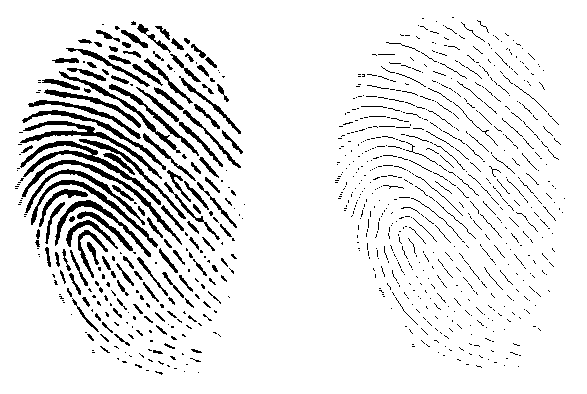
\includegraphics[scale=0.46]{thinning.png}
\caption{Primjer stanjivanja otiska prsta  \\ (preuzeto iz \cite{ blog:xxx})}
\end{figure}

Možemo zamisliti da je svaki crni slikovni element predstavljen s 1, dok je svaki bijeli predstavljen s vrijednošću 0. Zhang-Seunov algoritam djeluje nad crnim slikovnim elementima sa susjedstvom od 8 slikovnih elemenata. To automatski povlači da slikovni elementi na rubovima i u kutevima se ne razmatraju. Za svaki slikovni element koji se analizira, u nastavku je naveden redoslijed obilaska susjedstva. P1 je slikovni element koji se analizira.

\[
\begin{bmatrix}
P9 & P2 & P3 \\
P8 & \textbf{P1} & P4 \\
P7 & P6 & P5 \\
\end{bmatrix}
\]

U algoritmu se koriste dvije specifične vrijednosti:\newline
$A(P1)$ - broj prijelaza iz 0-1 odnosno iz bijelog slikovnog elementa u crni (analogno s prethodnom pretpostavkom o oznakama crnih i bijelih slikovnih elemenata) u sljedećem redoslijedu P2$\Rightarrow$P3$\Rightarrow$P4$\Rightarrow$P5$\Rightarrow$P6$\Rightarrow$P7$\Rightarrow$P8$\Rightarrow$P9$\Rightarrow$P2. Pogledamo li detaljnije matricu prijelaza, možemo uočiti da se krećemo u smjeru kazaljke na satu oko slikovnog elementa P1, pri čemu se P2 pojavljuje dva puta.\newline
$B(P1)$ = broj crnih slikovnih elemenata koji su susjedi od P1, odnosno drugim riječima koliko ima crnih slikovnih elemenata od P2 do P9.
\newline
\newline
Algoritam možemo razmatrati kroz dva koraka navedena u nastavku.
\newline
\textbf{Prvi korak}
\newline
U prvom koraku tražit ćemo P1 slikovne elemente koji zadovoljavaju 5 uvjeta. Ako P1 slikovni element zadovoljava svih 5 uvjeta, bit će postavljen kao bijeli slikovni element. Slikovni elementi se postavljaju kao bijeli nakon što se pronađu svi interesantni slikovni elementi jer u suprotnome neće biti konvergencije.

\begin{enumerate}
\item Slikovni element je crni (P1 = 1) i ima osam susjeda (dakle ne ubrajamo rubove i kuteve)
\item Broj susjednih crnih slikovnih elemenata  za P1 je najmanje 2 a najviše 6, odnosno $2\leq B(P1)\leq6$
\item Broj prijelaza iz bijelog u crni slikovni element oko P1 je jednak 1. Dakle, $A(P1) = 1$
\item P2, P4 ili P6 mora biti bijeli slikovni element (jednak 0)
\item P4, P6 ili P8 mora biti bijeli slikovni element (jednak 0)
\end{enumerate}
Svi P1 slikovni elementi koji zadovoljavaju gornjih 5 uvjeta se postavljaju kao bijeli, odnosno vrši se stanjivanje.
\newline
\textbf{Drugi korak}
\\
Prva tri dijela drugog koraka identični su kao u prethodnom koraku. Četvrti i peti korak su nešto razlikuju, kao što se može vidjeti u nastavku.

\begin{enumerate}
\item Slikovni element je crni (P1 = 1) i ima osam susjeda (dakle ne ubrajamo rubove i kuteve)
\item Broj susjednih crnih slikovnih elemenata za P1 je najmanje 2 a najviše 6, odnosno $2\leq B(P1)\leq6$
\item Broj prijelaza iz bijelog u crni slikovni element oko P1 je jednak 1. Dakle, $A(P1) = 1$
\item P2, P4 ili \textbf{P8} mora biti bijeli slikovni element (jednak 0)
\item \textbf{P2}, P6 ili P8 mora biti bijeli slikovni element (jednak 0)
\end{enumerate}

Identično, svi P1 slikovni elementi koji zadovoljavaju ovih 5 uvjeta se postavljaju kao bijeli, ali tek nakon što su pohranjeni slikovni elementi koji zadovoljavaju kriterije. Prvi i drugi korak se ponavljaju dokle god se slikovni elementi više ne mijenjanju.


\section{Interpolacija}
Kako duboki model na ulazu mreže za klasifikaciju rukom pisanih identifikatora očekuje slike istih dimenzija, a svaka od znamenki je varirajuće širine i visine potreban je postupak skaliranja odnosno interpolacije ulazne slike na željene dimenzije ulaza u mrežu. U tu svrhu u ovome radu implementirana je metoda interpolacije na temelju najbližeg susjeda \engl{Nearest-neighbor interpolation}. Sama interpolacija jest problem aproksimacije vrijednosti funkcije za nepoznatu točku u nekom prostoru kada je dana vrijednost iste funkcije u točkama oko te točke (za susjedne točke). Algoritam najbližeg susjeda odabire vrijednost koju poprima najbliža točka, dajući tako po dijelovima konstantne interpolante. Algoritam je dosta jednostavan i često u praksi korišten.

\begin{figure}[h]
\centering
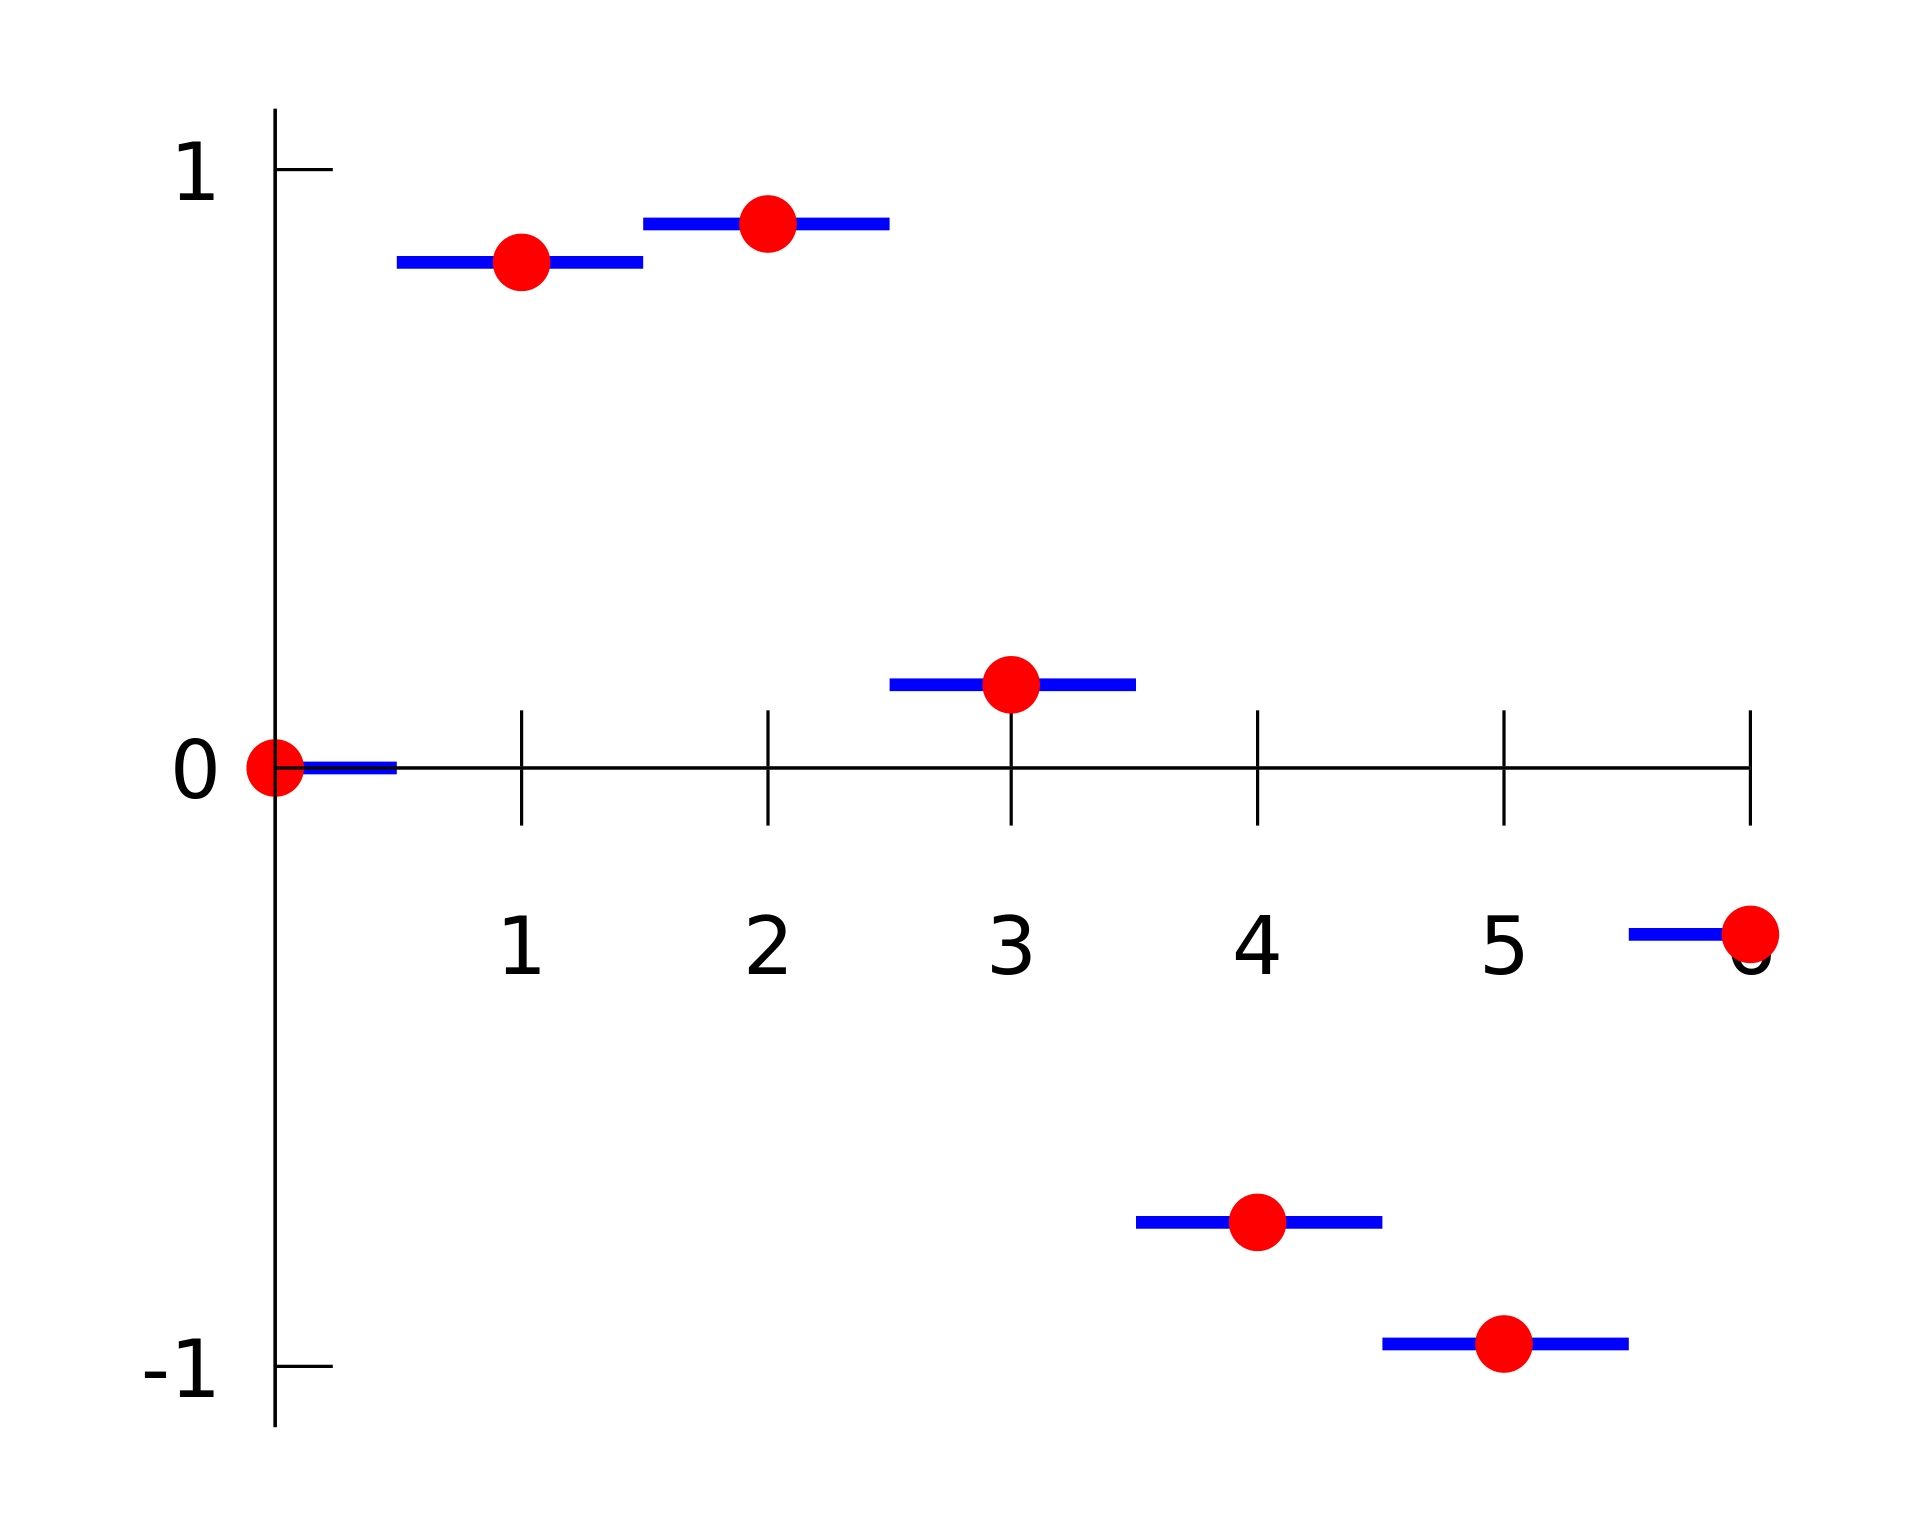
\includegraphics[scale=0.12]{n_n_interpolation.png}
\caption{Prikaz interpolacije metodom najbližeg susjeda \\ (preuzeto iz \cite{interpolation:xxx}}
\end{figure}
\section{Translacija}
Ulazne slike nakon skaliranja mogu se centrirati tako da se izračuna centar mase slikovnih elemenata koji čine konturu pojedine znamenke. Nakon izračuna centra mase konture znamenke (u ovome radu konturu čine bijeli slikovni elementi dok je pozadina crne boje), slika se translatira tako da je pozicija točke koja predstavlja centar mase u središtu skalirane slike. Ista metoda se koristi i u \textit{MNIST}-u, javno dostupnoj bazi rukom pisanih brojeva.
\section{Pronalazak povezanih komponenti}
Nakon obrade pojedine ulazne slike na kojoj se nalaze rukom pisani identifikatori potrebno je pronaći granične okvire oko svih znamenaka koje se pojavljuju na slici. Nakon pronalaska svih graničnih okvira, svaki okvir se smatra jednom ulaznom slikom za mrežu. Kako bi mreža uspješno mogla klasificirati pojedinu znamenku bitno je da što reprezentativnije pronađemo znamenke koje se nalaze na pojedinoj slici. Kako bismo to postigli koristi se efikasna metoda pronalaska povezanih komponenti \engl{Connected Component Labelling}. Upravo zato što sama metoda pronalazi povezane komponente, vrlo je bitno da dilatacijom dobivamo stvarne, neisprekidane konture znamenaka ili u suprotnom ćemo neprecizno pronalaziti granične okvire. Zbog toga nakon pronalaska graničnih okvira, slijedi niz dodatnih analiza. Jedna od njih jest  vertikalna analiza udaljenosti pojedinih graničnih okvira. Ako su dva granična okvira iste širine, te su neznatno vertikalno udaljeni jedan od drugoga, spajamo ih u jedan okvir kao uniju dosadašnjih graničnih okvira. Pretpostavka se tijekom testiranja implementiranog sustava pokazala vrlo korisnom, odnosno dovela jest do smanjenja broja pogrešno označenih graničnih okvira. Više o korištenim analizama detaljnije je opisano u nastavku. \newline\newline
U kontekstu analize algoritma u nastavku labeliranjem se smatra pridjeljivanje određene vrijednosti slikovnom elementu. Dakle, problem se svodi na labeliranje povezanih regija na slici. Cilj jest po završetku algoritma da povezane regije imaju iste labele. Klasični algoritam je osmišljen još u prošlom stoljeću, 1966. godine dizajnirali su ga Rosenfeld i Pfalz. Algoritam koristi strukturu \textit{union find} za rješavanje navedenog problema. Struktura \textit{union find} ima primjene u teoriji grafova za efikasno ispitivanje povezanosti čvorova u grafu. Sama struktura podržava spajanje dviju grupa i upit jesu li neka dva elementa u istoj grupi. Svaka grupa je stablo gdje je korijen zastupnik te grupe. Spajanje dviju grupa vršimo tako da zastupnika grupe prvog elementa spojimo kao dijete zastupnika drugog elementa. Kako bismo se riješili dugih lanaca ovdje možemo ubaciti provjeru koja u $50\%$ slučajeva zamijeni ta dva elementa. Da bismo provjerili jesu li 2 elementa u istoj grupi, moramo usporediti njihove zastupnike, odnosno korijene njihovih stabala. Prilikom traženja zastupnika možemo svu njegovu djecu koju prođemo spojiti direktno na njega. Zbog ovih dviju optimizacija obje operacije (\textit{union}, \textit{find}) imaju amortiziranu $\mathcal{O}(1)$ složenost.
\\
\\
\textbf{Algoritam}:
U prvom prolazu algoritma provjeravamo svaki slikovni element jednog po jednog, krenuvši od gornjeg lijevog ugla do donjeg desnog ugla.
\begin{figure}[h]
	\begin{center}
		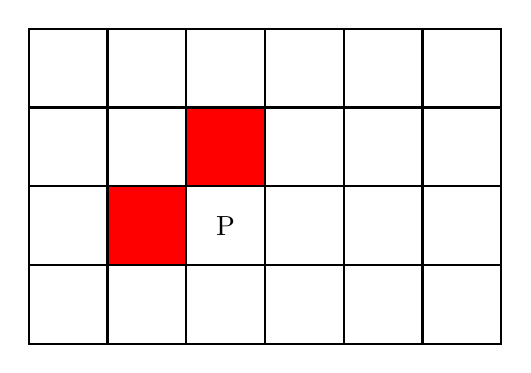
\begin{tikzpicture}
		[%%%%%%%%%%%%%%%%%%%%%%%%%%%%%%
		box/.style={rectangle,draw=black,thick, minimum size=1cm},
		]%%%%%%%%%%%%%%%%%%%%%%%%%%%%%%
		
		\foreach \x in {0,1,...,5}{
			\foreach \y in {0,1,...,3}
			\node[box] at (\x,\y){};
		}
		\node[box,fill=red] at (1,1){};
		\node[box,fill=red ] at (2,2){};
		\node at (2,1) {P};
		\end{tikzpicture}
	\end{center}
\caption{Prikaz slikovnih elemenata koji se razmatraju prilikom pronalaska povezanih komponenti}
\end{figure}

Razmatramo li slikovni element P, provjeravamo samo crvene slikovne elemente. Tako, u svakom trenutku izvođenja algoritma, u memoriji moramo imati samo dva retka slikovnih elemenata slike.
\begin{enumerate}
\item Provjeravamo je li trenutni slikovni element interesantan za razmatranje. Ako pripada pozadini, slikovni element ignoriramo i pomičemo se slijedno na idući. Ako pripada prednjem planu, krećemo na idući korak.
\item Dohvaćamo labele slikovnih elemenata iznad i lijevo od slikovnog elementa P. Pohranjujemo vrijednosti u varijable (nazovimo te varijable A i B).
\item Ako slikovni element iznad i/ili lijevo nije element pozadine, krećemo na idući korak. Inače, ako su oba slikovna elementa, elementi pozadine, ne možemo dohvatiti labele i kreiramo novu labelu te je pohranjujemo u A i B.
\item Uspoređujemo vrijednosti u varijablama A i B. Manju vrijednost pohranjujemo kao labelu slikovnog elementa P.
\item Pretpostavimo da imamo situaciju u kojoj slikovni element iznad ima labelu A i slikovni element lijevo ima labelu B. No, očito jest da su te dvije labele povezane (povezuje ih trenutni slikovni element P).
\begin{figure}[h]
\begin{center}
	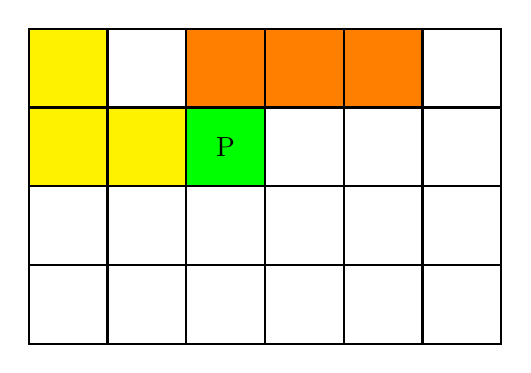
\begin{tikzpicture}
	[%%%%%%%%%%%%%%%%%%%%%%%%%%%%%%
	box/.style={rectangle,draw=black,thick, minimum size=1cm},
	]%%%%%%%%%%%%%%%%%%%%%%%%%%%%%%
	
	\foreach \x in {0,1,...,5}{
		\foreach \y in {0,1,...,3}
		\node[box] at (\x,\y){};
	}
	\node[box,fill=orange] at (2,3){};
	\node[box,fill=orange ] at (3,3){};
	\node[box,fill=orange ] at (4,3){};
	\node[box,fill=green ] at (2,2) {P};
	\node[box,fill=yellow ] at (1,2){};
	\node[box,fill=yellow ] at (0,2){};
	\node[box,fill=yellow ] at (0,3){};
	
	
	\end{tikzpicture}
\end{center}
\caption{Povezane komponente označene različitim labelama}
\end{figure}
Tada moramo pohraniti informaciju da su labele A i B jednake. Tu se u igru uključuje gore spomenuta struktura \textit{union find}. Postavljamo labelu A kao dijete od labele B. Ta informacija će nam kasnije biti korisna u drugom prolazu algoritma kako bi "počistili nered". Bitno jest napomenuti da manja labela se pridružuje slikovnom elementu P, a veća labela postaje dijete od manje labele. Inicijalno je svaka nova labela svoj zastupnik te prolazom kroz slikovne elemente može postati dijete neke druge labele.
\item Prelazimo na idući slikovni element.
\end{enumerate}
U drugom prolazu algoritma također idemo slikovni element po element, od gornjeg lijevog kuta do donjeg desnog.
\begin{enumerate}
\item Provjeravamo za slikovni element je li zastupnik u strukturi \textit{union find}. Ako jest, idemo na idući slikovni element i ponavljamo postupak.
\item Inače, pratimo poveznicu do zastupnika grupe. Kada smo pronašli zastupnika grupe, dodjeljujemo nađenu labelu trenutnom slikovnom elementu.
\end{enumerate}
\subsection{Primjer rada algoritma}
\begin{figure}[H]
	Pretpostavimo da promatramo binarnu sliku \ref{fig:binary_image} gdje 1 označava bijeli slikovni element, dok 0 označava crni. Zanima nas labeliranje bijelih slikovnih elemenata.
\begin{center}
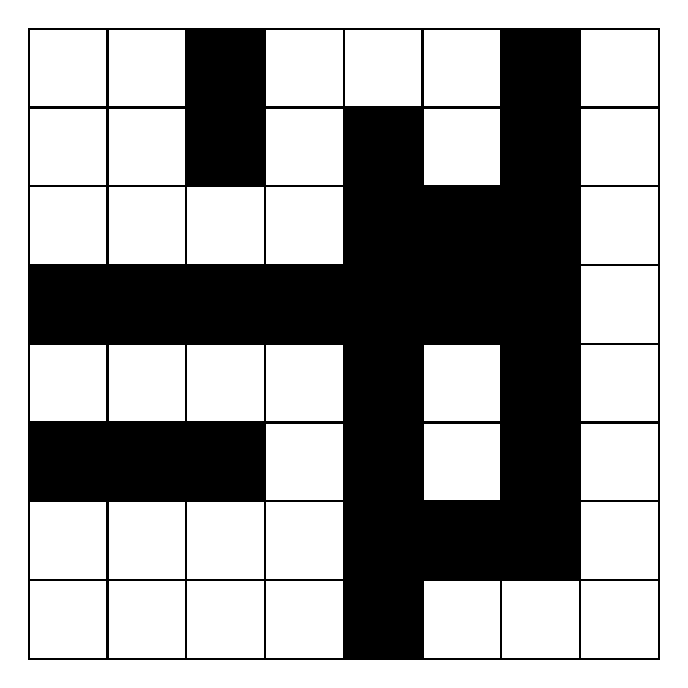
\begin{tikzpicture}
[%%%%%%%%%%%%%%%%%%%%%%%%%%%%%%
box/.style={rectangle,draw=black,thick, minimum size=1cm},
]%%%%%%%%%%%%%%%%%%%%%%%%%%%%%%

\foreach \x in {0,1,...,7}{
\foreach \y in {0,1,...,7}
\node[box] at (\x,\y){};
}
\node[box,fill=black] at (0,2){};
\node[box,fill=black ] at (0,4){};
\node[box,fill=black] at (1,2){};
\node[box,fill=black ] at (1,4){};
\node[box,fill=black] at (2,2){};
\node[box,fill=black ] at (2,4){};
\node[box,fill=black] at (2,6){};
\node[box,fill=black ] at (2,7){};
\node[box,fill=black] at (3,4){};
\node[box,fill=black ] at (4,0){};
\node[box,fill=black ] at (4,1){};
\node[box,fill=black ] at (4,2){};
\node[box,fill=black ] at (4,3){};
\node[box,fill=black ] at (4,4){};
\node[box,fill=black ] at (4,5){};
\node[box,fill=black ] at (4,6){};
\node[box,fill=black ] at (5,1){};
\node[box,fill=black ] at (5,4){};
\node[box,fill=black ] at (5,5){};
\node[box,fill=black ] at (6,1){};
\node[box,fill=black ] at (6,2){};
\node[box,fill=black ] at (6,3){};
\node[box,fill=black ] at (6,4){};
\node[box,fill=black ] at (6,5){};
\node[box,fill=black ] at (6,6){};
\node[box,fill=black ] at (6,7){};
\end{tikzpicture}
\end{center}
\caption{Binarna slika za demonstraciju pronalaska povezanih komponenti}
\label{fig:binary_image}
\end{figure}
Prva specifična situacija se dešava kada promatramo treći redak i četvrti stupac $(3,4)$ kao što je prikazano na slici \ref{fig:different_labels}. Imamo slikove elemente i lijevo i iznad spomenutog slikovnog elementa, i oba imaju različite labele. Kao što je prethodno spomenuto, uzimamo labelu s manjom vrijednošću i postavljamo je na poziciju $(3,4)$, dakle labelu s vrijednošću 1. Također, labelu $2$ (numerički veća labela) pohranjujemo kao dijete od labele $1$ koristeći strukturu \textit{union find}. Dakle, u strukturi \textit{union find} nakon obrade ovog slikovnog elementa imamo pohranjeno da je labela $2$ dijete od labele $1$.
\begin{figure}[H]
\begin{center}
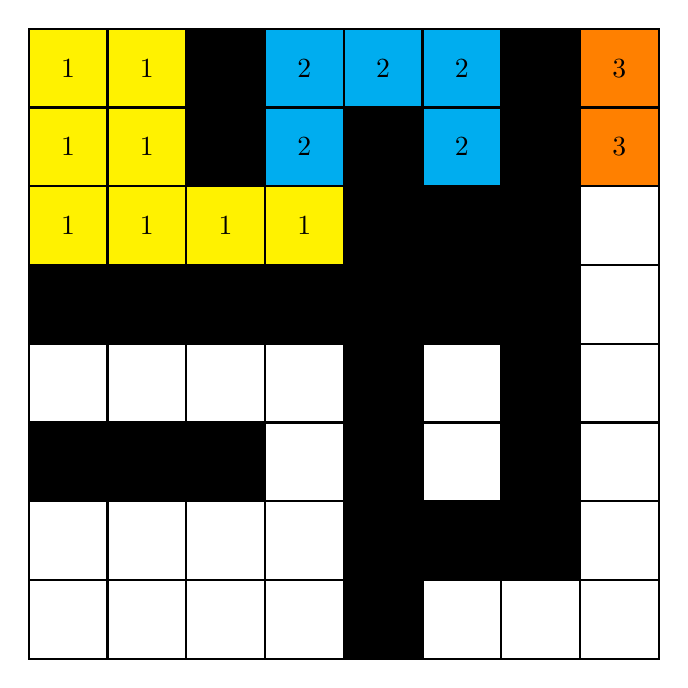
\begin{tikzpicture}
[%%%%%%%%%%%%%%%%%%%%%%%%%%%%%%
box/.style={rectangle,draw=black,thick, minimum size=1cm},
]%%%%%%%%%%%%%%%%%%%%%%%%%%%%%%

\foreach \x in {0,1,...,7}{
\foreach \y in {0,1,...,7}
\node[box] at (\x,\y){};
}
\node[box,fill=yellow] at (0,7){1};
\node[box,fill=yellow] at (0,6){1};
\node[box,fill=yellow] at (0,5){1};
\node[box,fill=yellow ] at (1,7){1};
\node[box,fill=yellow] at (1,6){1};
\node[box,fill=yellow ] at (1,5){1};
\node[box,fill=yellow] at (2,5){1};
\node[box,fill=yellow ] at (3,5){1};

\node[box,fill=cyan] at (3,7){2};
\node[box,fill=cyan ] at (3,6){2};
\node[box,fill=cyan] at (4,7){2};
\node[box,fill=cyan ] at (5,7){2};
\node[box,fill=cyan] at (5,6){2};


\node[box,fill=orange] at (7,7){3};
\node[box,fill=orange ] at (7,6){3};

\node[box,fill=black] at (0,2){};
\node[box,fill=black ] at (0,4){};
\node[box,fill=black] at (1,2){};
\node[box,fill=black ] at (1,4){};
\node[box,fill=black] at (2,2){};
\node[box,fill=black ] at (2,4){};
\node[box,fill=black] at (2,6){};
\node[box,fill=black ] at (2,7){};
\node[box,fill=black] at (3,4){};
\node[box,fill=black ] at (4,0){};
\node[box,fill=black ] at (4,1){};
\node[box,fill=black ] at (4,2){};
\node[box,fill=black ] at (4,3){};
\node[box,fill=black ] at (4,4){};
\node[box,fill=black ] at (4,5){};
\node[box,fill=black ] at (4,6){};
\node[box,fill=black ] at (5,1){};
\node[box,fill=black ] at (5,4){};
\node[box,fill=black ] at (5,5){};
\node[box,fill=black ] at (6,1){};
\node[box,fill=black ] at (6,2){};
\node[box,fill=black ] at (6,3){};
\node[box,fill=black ] at (6,4){};
\node[box,fill=black ] at (6,5){};
\node[box,fill=black ] at (6,6){};
\node[box,fill=black ] at (6,7){};
\end{tikzpicture}
\end{center}
\caption{Primjer slikovnog elementa $(3, 4)$ koji povezuje različito labelirane komponente}
\label{fig:different_labels}
\end{figure}
\begin{figure}[H]
	Pratimo li dalje korake prethodno opisanog prvog prolaza algoritma naposljetku dobivamo strukturu kao na slici \ref{fig:first_step}.
\begin{center}
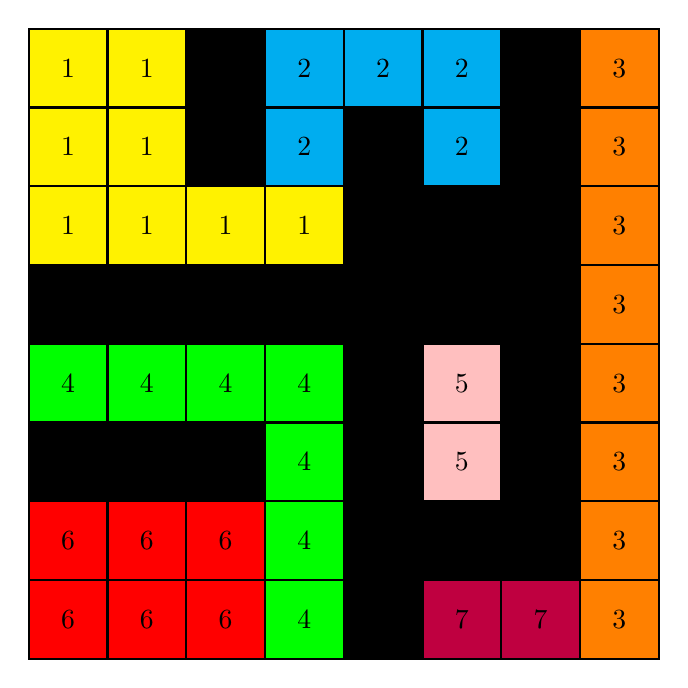
\begin{tikzpicture}
[%%%%%%%%%%%%%%%%%%%%%%%%%%%%%%
box/.style={rectangle,draw=black,thick, minimum size=1cm},
]%%%%%%%%%%%%%%%%%%%%%%%%%%%%%%

\foreach \x in {0,1,...,7}{
\foreach \y in {0,1,...,7}
\node[box] at (\x,\y){};
}
\node[box,fill=yellow] at (0,7){1};
\node[box,fill=yellow] at (0,6){1};
\node[box,fill=yellow] at (0,5){1};
\node[box,fill=yellow ] at (1,7){1};
\node[box,fill=yellow] at (1,6){1};
\node[box,fill=yellow ] at (1,5){1};
\node[box,fill=yellow] at (2,5){1};
\node[box,fill=yellow ] at (3,5){1};

\node[box,fill=cyan] at (3,7){2};
\node[box,fill=cyan ] at (3,6){2};
\node[box,fill=cyan] at (4,7){2};
\node[box,fill=cyan ] at (5,7){2};
\node[box,fill=cyan] at (5,6){2};


\node[box,fill=orange] at (7,7){3};
\node[box,fill=orange ] at (7,6){3};
\node[box,fill=orange] at (7,5){3};
\node[box,fill=orange ] at (7,4){3};
\node[box,fill=orange] at (7,3){3};
\node[box,fill=orange] at (7,2){3};
\node[box,fill=orange] at (7,1){3};
\node[box,fill=orange] at (7,0){3};

\node[box,fill=purple] at (5,0){7};
\node[box,fill=purple] at (6,0){7};

\node[box,fill=red] at (0,0){6};
\node[box,fill=red] at (0,1){6};
\node[box,fill=red] at (1,0){6};
\node[box,fill=red] at (1,1){6};
\node[box,fill=red] at (2,0){6};
\node[box,fill=red] at (2,1){6};

\node[box,fill=green] at (0,3){4};
\node[box,fill=green] at (1,3){4};
\node[box,fill=green] at (2,3){4};
\node[box,fill=green] at (3,3){4};
\node[box,fill=green] at (3,2){4};
\node[box,fill=green] at (3,1){4};
\node[box,fill=green] at (3,0){4};

\node[box,fill=pink] at (5,3){5};
\node[box,fill=pink] at (5,2){5};

\node[box,fill=black] at (0,2){};
\node[box,fill=black ] at (0,4){};
\node[box,fill=black] at (1,2){};
\node[box,fill=black ] at (1,4){};
\node[box,fill=black] at (2,2){};
\node[box,fill=black ] at (2,4){};
\node[box,fill=black] at (2,6){};
\node[box,fill=black ] at (2,7){};
\node[box,fill=black] at (3,4){};
\node[box,fill=black ] at (4,0){};
\node[box,fill=black ] at (4,1){};
\node[box,fill=black ] at (4,2){};
\node[box,fill=black ] at (4,3){};
\node[box,fill=black ] at (4,4){};
\node[box,fill=black ] at (4,5){};
\node[box,fill=black ] at (4,6){};
\node[box,fill=black ] at (5,1){};
\node[box,fill=black ] at (5,4){};
\node[box,fill=black ] at (5,5){};
\node[box,fill=black ] at (6,1){};
\node[box,fill=black ] at (6,2){};
\node[box,fill=black ] at (6,3){};
\node[box,fill=black ] at (6,4){};
\node[box,fill=black ] at (6,5){};
\node[box,fill=black ] at (6,6){};
\node[box,fill=black ] at (6,7){};
\end{tikzpicture}
\end{center}
\caption{Labele nakon prvog prolaza algoritma}
\label{fig:first_step}
\end{figure}

\begin{figure}[H]
	Nakon završenog prvog koraka labela s vrijednošću $2$ je dijete labele $1$, labela $6$ je dijete labele $4$ i labela $7$ je dijete labele $3$.
	U idućem prolazu na temelju odnosa dijete-roditelj vršimo filtriranje, kao što je prethodno opisano, te u konačnici imamo situaciju kao na slici \ref{fig:second_step}.
\begin{center}
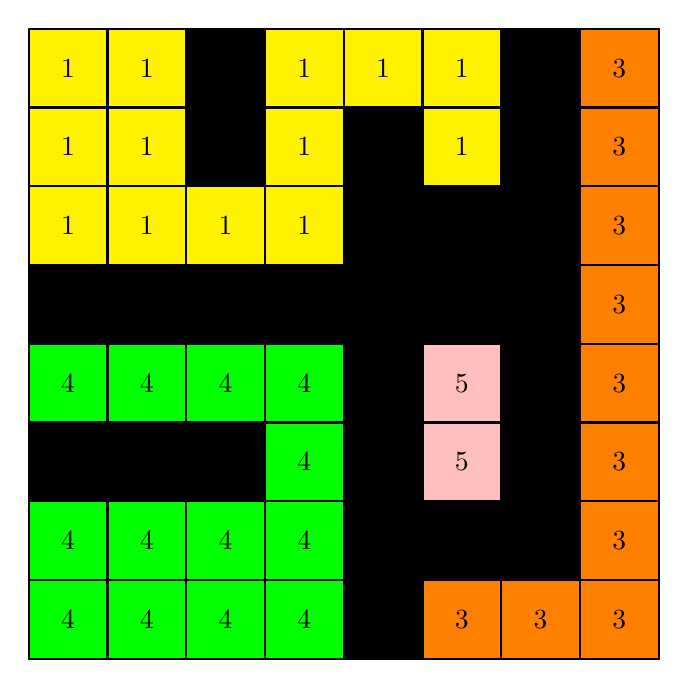
\begin{tikzpicture}
[%%%%%%%%%%%%%%%%%%%%%%%%%%%%%%
box/.style={rectangle,draw=black,thick, minimum size=1cm},
]%%%%%%%%%%%%%%%%%%%%%%%%%%%%%%

\foreach \x in {0,1,...,7}{
\foreach \y in {0,1,...,7}
\node[box] at (\x,\y){};
}
\node[box,fill=yellow] at (0,7){1};
\node[box,fill=yellow] at (0,6){1};
\node[box,fill=yellow] at (0,5){1};
\node[box,fill=yellow ] at (1,7){1};
\node[box,fill=yellow] at (1,6){1};
\node[box,fill=yellow ] at (1,5){1};
\node[box,fill=yellow] at (2,5){1};
\node[box,fill=yellow ] at (3,5){1};

\node[box,fill=yellow] at (3,7){1};
\node[box,fill=yellow ] at (3,6){1};
\node[box,fill=yellow] at (4,7){1};
\node[box,fill=yellow ] at (5,7){1};
\node[box,fill=yellow] at (5,6){1};


\node[box,fill=orange] at (7,7){3};
\node[box,fill=orange ] at (7,6){3};
\node[box,fill=orange] at (7,5){3};
\node[box,fill=orange ] at (7,4){3};
\node[box,fill=orange] at (7,3){3};
\node[box,fill=orange] at (7,2){3};
\node[box,fill=orange] at (7,1){3};
\node[box,fill=orange] at (7,0){3};

\node[box,fill=orange] at (5,0){3};
\node[box,fill=orange] at (6,0){3};

\node[box,fill=green] at (0,0){4};
\node[box,fill=green] at (0,1){4};
\node[box,fill=green] at (1,0){4};
\node[box,fill=green] at (1,1){4};
\node[box,fill=green] at (2,0){4};
\node[box,fill=green] at (2,1){4};

\node[box,fill=green] at (0,3){4};
\node[box,fill=green] at (1,3){4};
\node[box,fill=green] at (2,3){4};
\node[box,fill=green] at (3,3){4};
\node[box,fill=green] at (3,2){4};
\node[box,fill=green] at (3,1){4};
\node[box,fill=green] at (3,0){4};

\node[box,fill=pink] at (5,3){5};
\node[box,fill=pink] at (5,2){5};

\node[box,fill=black] at (0,2){};
\node[box,fill=black ] at (0,4){};
\node[box,fill=black] at (1,2){};
\node[box,fill=black ] at (1,4){};
\node[box,fill=black] at (2,2){};
\node[box,fill=black ] at (2,4){};
\node[box,fill=black] at (2,6){};
\node[box,fill=black ] at (2,7){};
\node[box,fill=black] at (3,4){};
\node[box,fill=black ] at (4,0){};
\node[box,fill=black ] at (4,1){};
\node[box,fill=black ] at (4,2){};
\node[box,fill=black ] at (4,3){};
\node[box,fill=black ] at (4,4){};
\node[box,fill=black ] at (4,5){};
\node[box,fill=black ] at (4,6){};
\node[box,fill=black ] at (5,1){};
\node[box,fill=black ] at (5,4){};
\node[box,fill=black ] at (5,5){};
\node[box,fill=black ] at (6,1){};
\node[box,fill=black ] at (6,2){};
\node[box,fill=black ] at (6,3){};
\node[box,fill=black ] at (6,4){};
\node[box,fill=black ] at (6,5){};
\node[box,fill=black ] at (6,6){};
\node[box,fill=black ] at (6,7){};
\end{tikzpicture}
\end{center}
\caption{Pronađene povezane komponente}
\label{fig:second_step}
\end{figure}
Ovo je upravo rezultat koji smo inicijalno željeli dobiti, te možemo uočiti kako je svaka povezana regija poprimila specifičnu labelu koja je predstavnik same regije.

\chapter{Izgrađeni sustav}
Sustav je implementiran koristeći programski jezik \textit{Java} i radni okvir za duboko učenje \textit{Deeplearning4j}. Kao što je prethodno spomenuto svaka od učitanih slika prolazi kroz faze pretvorbe u sive nijanse, binarizacije odnosno odvajanja prednjeg plana od pozadine, dilatacije, interpolacije metodom najbližeg susjeda te centriranja metodom centra mase. Tako transformirana slika se šalje kao ulaz metodi koja je zadužena za pronalazak povezanih kontura na slici koje kasnije koristimo za pronalazak okvira oko pojedine znamenke. Nakon pronalaska pojedinih okvira slike se šalju na ulaz konvolucijske duboke neuronske mreže. U skupu za učenje duboke konvolucijske neuronske mreže bilo je $2371$ slika, dok se skup za testiranje sastojao od $402$ slike. Baza jest izgrađena od rukom pisanih identifikatora pisanih od strane više različitih osoba. Mreža je imala $6$ slojeva i ukupno $1385130$ parametara. Učenje je provedeno kroz $30$ epoha, u mini-grupama \engl{mini-batch} od po $54$ uzorka. Svaka od slika se prethodno spomenutom metodom interpolacije skalirala na dimenzije 28x28, što je ujedno i dimenzija ulaznog sloja. Za dodjeljivanje inicijalnih težina korištena je Xavierova inicijalizacija. Kod Xavierove inicijalizacije težine se inicijaliziraju iz normalne distribucije:
\begin{equation}
W_{i, j} \sim \mathcal{N}(0, \frac{2}{n_{in} + n_{out}})\quad \textrm{ili} \quad W_{i, j} \sim \mathcal{N}(0, \frac{0}{n_{in}}),
\end{equation}
gdje je $n_{in}$ broj ulaza neurona, a $n_{out}$ broj izlaza neurona. Konkretno u implementaciji je korištena prva varijanta. U praksi se često za inicijalizaciju težina koristi Xavierova inicijalizacija.
Za učenje mreže korišten je stohastički gradijenti spust \engl{Stochastic gradient descent} (SGD) s Nesterovim momentom. Učenje s momentom koristi se za ubrzavanje učenja kod šumovite procjene gradijenta i kod malih ali konzistentnih gradijenata. Postupak akumulira eksponencijalno umanjujući prosjek prethodno izračunatih gradijenata i nastavlja u tome smjeru.
\begin{equation}
\bm{v} \leftarrow \alpha \cdot \bm{v} - \epsilon \cdot \nabla_{\bm{\theta}}(\frac{1}{m} \sum_{i=1}^{m}L(f(\bm{x}^{(i)}; \bm{\theta}), y^i )
\end{equation}
\begin{equation}
\bm{\theta} \leftarrow \bm{\theta} + \bm{v},
\end{equation}
pri čemu $\bm{v}$ predstavlja eksponencijalno umanjujući prosjek prethodnih gradijenata, $\alpha \in [0, 1)$ predstavlja brzinu umanjivanja odnosno govori koliko je relevantan prethodno izračunati prosjek, $\epsilon \in [0, 1)$ je stopa učenja. $L$ je funkcija gubitka dok je $f(\bm{x}; \bm{\theta})$ predviđeni izlaz našeg modela za neki uzorak $\bm{x}$ iz skupa za učenje. Iz jednadžbe osvježavanja parametara modela jasno je da parametrima $\alpha$ i $\epsilon$ možemo korelirati utjecaj prethodnih gradijenata odnosno trenutno izračunatih gradijenata. Što je manji $\alpha$ u odnosu na $\epsilon$, to je manji utjecaj prethodnih gradijenata na smjer ažuriranja.
Modifikacijom osnovnog algoritma učenja s momentom dolazimo do Nesterovog momenta koji parametra ažurira na sljedeći način:

\begin{equation}
\bm{v} \leftarrow \alpha \cdot \bm{v} - \epsilon \cdot \nabla_{\bm{\theta}}(\frac{1}{m} \sum_{i=1}^{m}L(f(\bm{x}^{(i)}; \bm{\theta} + \alpha \bm{v}), y^i )
\end{equation}
\begin{equation}
\bm{\theta} \leftarrow \bm{\theta} + \bm{v},
\end{equation}
Dakle, razlika u odnosu na osnovni algoritam jest u tome da gradijent računamo u parametrima koji odgovaraju $\bm{\theta} + \alpha \bm{v}$. Nadalje klasično računamo prosjek gradijenata i radimo korekciju izvornih parametara izgrađenog modela. Dodatno, u izgrađenom modelu koristi se L2 regularizacija s parametrom $\lambda = 0.0005$.

\begin{figure}[h]
\centering
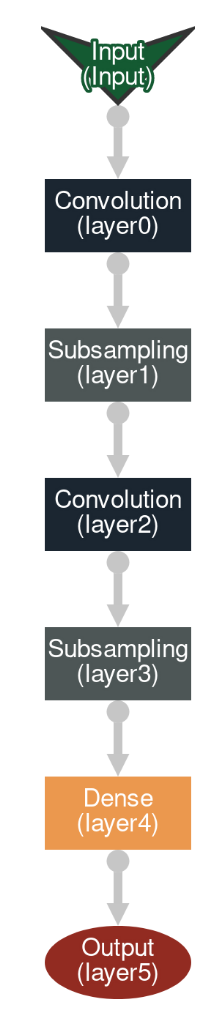
\includegraphics[scale=0.4]{arhitektura_neuronske_mreze.png}
\caption{Arhitektura izgrađenog konvolucijskog modela}
\label{fig:arhitecture}
\end{figure}

Na slici \ref{fig:arhitecture} možemo vidjeti arhitekturu izgrađene konvolucijske neuronske mreže. Nakon ulaznog sloja 28x28x1 slijedi konvolucijski sloj s jezgrom dimenzija [5, 5] i pomakom [1, 1], bez nadopunjavanja. Kao prijenosna odnosno aktivacijska funkcija koristi se funkcija identiteta. Zatim slijedi sloj za sažimanje maksimalnom vrijednošću, koristi jezgru dimenzija [2, 2] s pomakom [2, 2], također bez nadopunjavanja. Idući sloj je opet konvolucijski s jezgrom dimenzija [5, 5] i pomakom [1, 1], no kao aktivacijsku funkciju koristi ispravljenu linearnu funkciju ReLu. Slijedi identični sloj za sažimanje maksimalnom vrijednošću, te na kraju potpuno povezani sloj s ispravljenom linearnom aktivacijskom funkcijom koji se veže na 10 izlaza (za svaku znamenku imamo po jedan izlaz).

\begin{figure}[h]
\centering
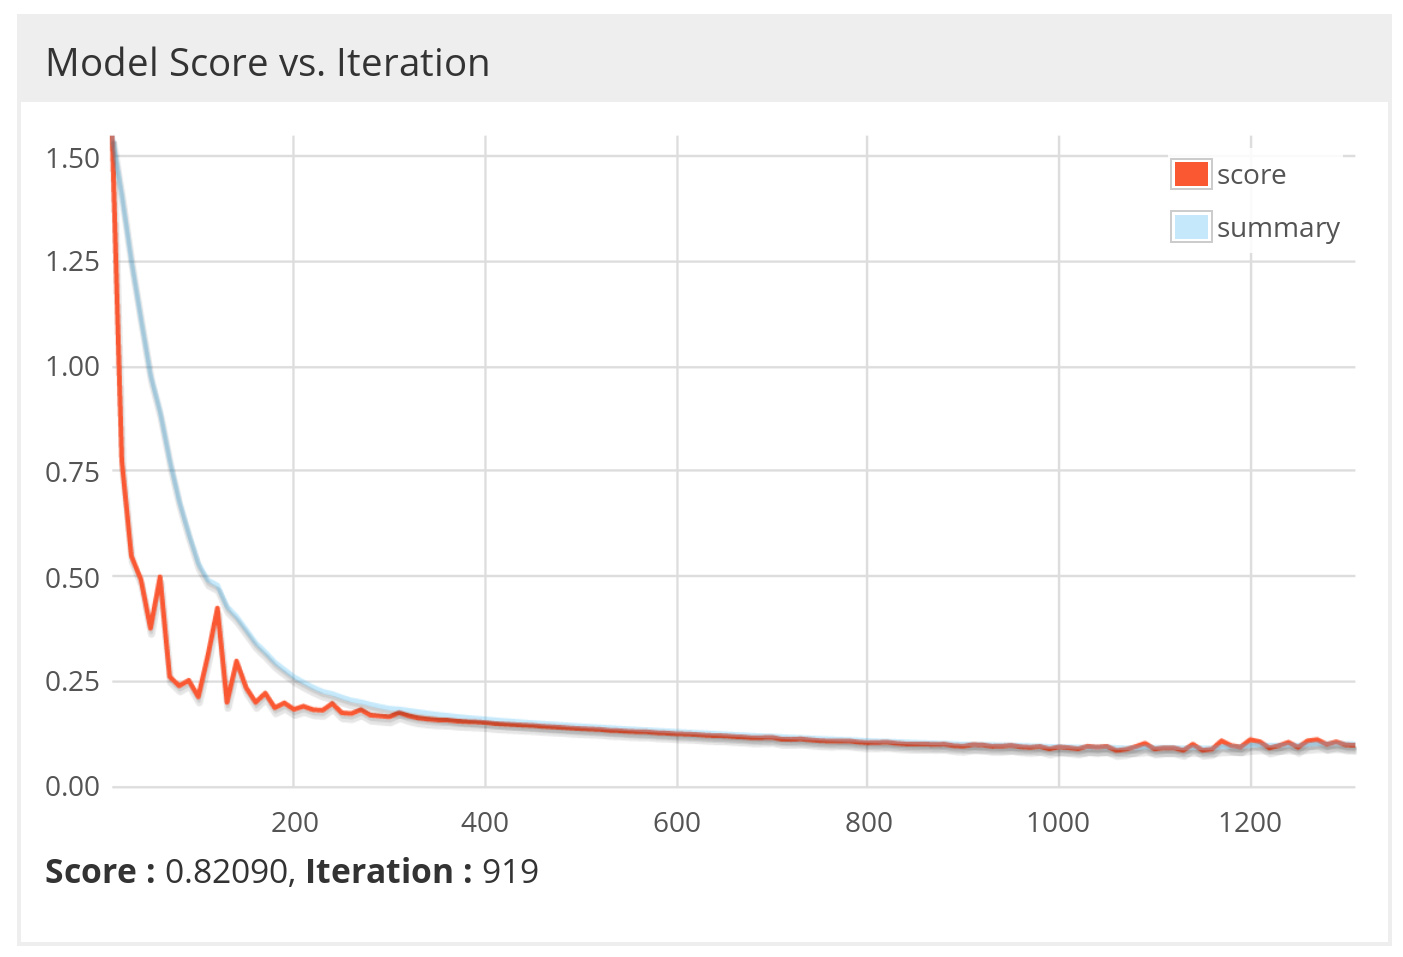
\includegraphics[scale=0.3]{funkcija_gubitka.png}
\caption{Vrijednost funkcije gubitka kroz iteracije}
\end{figure}

\begin{figure}[h]
\centering
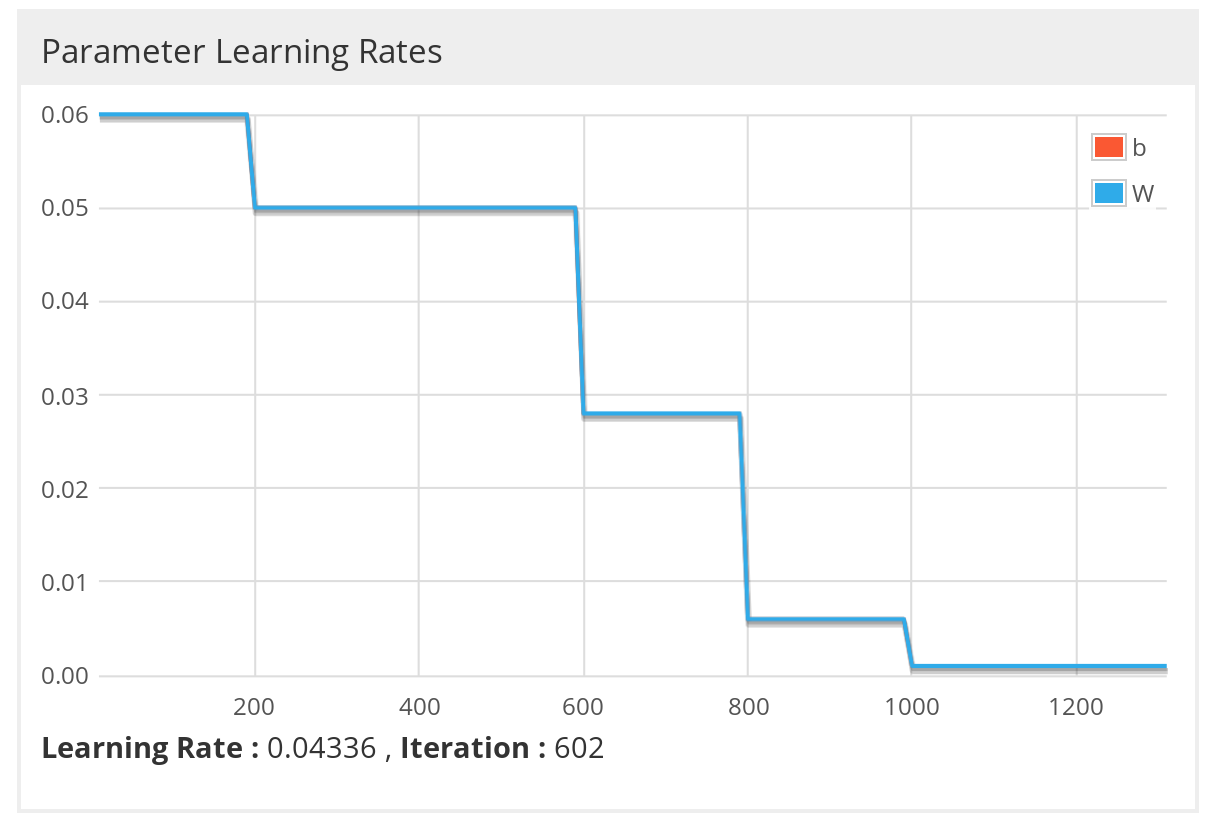
\includegraphics[scale=0.28]{learning_rate.png}
\caption{Stope učenja kroz iteracije}
\end{figure}


Kako bi procijenili koliko je klasifikator dobar koristimo četiri osnovne mjere evaluacije: točnost \engl{accuracy}, preciznost \engl{precision}, odziv \engl{recall} i F1 mjeru.
\newline
Točnost definiramo kao omjer ispravno klasificiranih primjera i ukupnog broja primjera:
$A_{cc} = \frac{TP + TN}{N} = \frac{TP + TN}{TP + TN + FP + FN}$.
\newline
Preciznost je definirana izrazom: $P = \frac{TP}{TP + FP}$.
\newline
Odziv je definiran omjerom broja primjera koje je klasifikator označio kao pozitivne i ukupnog broja pozitivnih primjera:
$R = \frac{TP}{TP + FN}$. Još se i naziva \textit{true positive rate}.
\newline
F1 mjeru definiramo kao harmonijsku sredinu između preciznosti i odziva:
$F1 = \frac{2}{\frac{1}{P} + \frac{1}{R}} = \frac{2PR}{P + R}$. Kako se svaka matrica dimenzija NxN može svesti na matricu dimenzija 2x2 za svaku od $N$ klasa (ukupno N matrica 2x2), navedene formule možemo koristiti za računanje mjera naše 10x10 matrice zabune i dobivamo rezultate kao u tablici \ref{tab:evaluation-matrix}.
\newline
Iz tablice evaluacije modela možemo primijetiti kako implementirani klasifikator na testnome skupu postiže gotovo 97\% za svaku od mjera.

\begin{table}[h]
\centering
\begin{tabular}{lllllllllll}
& \cellcolor[HTML]{FFFFFF}{\color[HTML]{333333} 0} & 1 & 2 & 3 & 4 & 5 & 6 & 7 & 8 & 9 \\ \cline{2-11}
\multicolumn{1}{l|}{0=0} & \multicolumn{1}{l|}{\cellcolor[HTML]{FFCB2F}39} & \multicolumn{1}{l|}{0} & \multicolumn{1}{l|}{0} & \multicolumn{1}{l|}{0} & \multicolumn{1}{l|}{0} & \multicolumn{1}{l|}{0} & \multicolumn{1}{l|}{0} & \multicolumn{1}{l|}{0} & \multicolumn{1}{l|}{1} & \multicolumn{1}{l|}{0} \\ \cline{2-11}
\multicolumn{1}{l|}{1=1} & \multicolumn{1}{l|}{0} & \multicolumn{1}{l|}{\cellcolor[HTML]{FFCB2F}41} & \multicolumn{1}{l|}{0} & \multicolumn{1}{l|}{0} & \multicolumn{1}{l|}{0} & \multicolumn{1}{l|}{0} & \multicolumn{1}{l|}{0} & \multicolumn{1}{l|}{0} & \multicolumn{1}{l|}{0} & \multicolumn{1}{l|}{0} \\ \cline{2-11}
\multicolumn{1}{l|}{2=2} & \multicolumn{1}{l|}{0} & \multicolumn{1}{l|}{0} & \multicolumn{1}{l|}{\cellcolor[HTML]{FFCB2F}40} & \multicolumn{1}{l|}{0} & \multicolumn{1}{l|}{0} & \multicolumn{1}{l|}{0} & \multicolumn{1}{l|}{0} & \multicolumn{1}{l|}{0} & \multicolumn{1}{l|}{0} & \multicolumn{1}{l|}{0} \\ \cline{2-11}
\multicolumn{1}{l|}{3=3} & \multicolumn{1}{l|}{0} & \multicolumn{1}{l|}{0} & \multicolumn{1}{l|}{0} & \multicolumn{1}{l|}{\cellcolor[HTML]{FFCB2F}37} & \multicolumn{1}{l|}{0} & \multicolumn{1}{l|}{0} & \multicolumn{1}{l|}{0} & \multicolumn{1}{l|}{0} & \multicolumn{1}{l|}{0} & \multicolumn{1}{l|}{3} \\ \cline{2-11}
\multicolumn{1}{l|}{4=4} & \multicolumn{1}{l|}{0} & \multicolumn{1}{l|}{0} & \multicolumn{1}{l|}{0} & \multicolumn{1}{l|}{0} & \multicolumn{1}{l|}{\cellcolor[HTML]{FFCB2F}40} & \multicolumn{1}{l|}{0} & \multicolumn{1}{l|}{0} & \multicolumn{1}{l|}{0} & \multicolumn{1}{l|}{0} & \multicolumn{1}{l|}{0} \\ \cline{2-11}
\multicolumn{1}{l|}{5=5} & \multicolumn{1}{l|}{0} & \multicolumn{1}{l|}{0} & \multicolumn{1}{l|}{0} & \multicolumn{1}{l|}{0} & \multicolumn{1}{l|}{0} & \multicolumn{1}{l|}{\cellcolor[HTML]{FFCB2F}36} & \multicolumn{1}{l|}{4} & \multicolumn{1}{l|}{0} & \multicolumn{1}{l|}{0} & \multicolumn{1}{l|}{0} \\ \cline{2-11}
\multicolumn{1}{l|}{6=6} & \multicolumn{1}{l|}{0} & \multicolumn{1}{l|}{0} & \multicolumn{1}{l|}{0} & \multicolumn{1}{l|}{0} & \multicolumn{1}{l|}{2} & \multicolumn{1}{l|}{0} & \multicolumn{1}{l|}{\cellcolor[HTML]{FFCB2F}38} & \multicolumn{1}{l|}{0} & \multicolumn{1}{l|}{0} & \multicolumn{1}{l|}{0} \\ \cline{2-11}
\multicolumn{1}{l|}{7=7} & \multicolumn{1}{l|}{0} & \multicolumn{1}{l|}{0} & \multicolumn{1}{l|}{0} & \multicolumn{1}{l|}{0} & \multicolumn{1}{l|}{0} & \multicolumn{1}{l|}{0} & \multicolumn{1}{l|}{0} & \multicolumn{1}{l|}{\cellcolor[HTML]{FFCB2F}41} & \multicolumn{1}{l|}{0} & \multicolumn{1}{l|}{0} \\ \cline{2-11}
\multicolumn{1}{l|}{8=8} & \multicolumn{1}{l|}{0} & \multicolumn{1}{l|}{0} & \multicolumn{1}{l|}{0} & \multicolumn{1}{l|}{0} & \multicolumn{1}{l|}{0} & \multicolumn{1}{l|}{0} & \multicolumn{1}{l|}{0} & \multicolumn{1}{l|}{0} & \multicolumn{1}{l|}{\cellcolor[HTML]{FFCB2F}40} & \multicolumn{1}{l|}{0} \\ \cline{2-11}
\multicolumn{1}{l|}{9=9} & \multicolumn{1}{l|}{0} & \multicolumn{1}{l|}{0} & \multicolumn{1}{l|}{0} & \multicolumn{1}{l|}{0} & \multicolumn{1}{l|}{3} & \multicolumn{1}{l|}{0} & \multicolumn{1}{l|}{0} & \multicolumn{1}{l|}{0} & \multicolumn{1}{l|}{0} & \multicolumn{1}{l|}{\cellcolor[HTML]{FFCB2F}37} \\ \cline{2-11}
\end{tabular}
\caption{Matrica zabune}
\label{tab:confusion-matrix}
\end{table}


\begin{table}[h]
\centering
\begin{tabular}{|c|
>{\columncolor[HTML]{FFCB2F}}c |}
\hline
Točnost & {\color[HTML]{333333} 0.9677} \\ \hline
Preciznost & 0.9694 \\ \hline
Odziv & 0.9675 \\ \hline
F1 & 0.9676 \\ \hline
\end{tabular}
\caption{Evaluacija modela}
\label{tab:evaluation-matrix}
\end{table}

Nakon implementacije sustava za obradu slike, pronalazak okvira oko znamenaka i sustava za klasifikaciju, implementirano je grafičko korisničko sučelje \engl{Graphical User Interface} koristeći \textit{Swing} koji pruža skup biblioteka za kreiranje GUI-a neovisno o platformi \engl{cross-platform}. \newline
Pokretanjem aplikacije korisnik unutar izbornika odabire direktorij sa slikama koje želi poluautomatski labelirati. Ako u direktoriju postoji slika, sustav prikazuje prvu na koju je naišao te dodatno pomoću prethodno opisanih metoda pronalazi okvire oko pojedinih znamenaka i dodjeljuje svakoj od znamenaka jednu od klasa. Korisnik ima mogućnost uređivati postojeće okvire, brisati, dodavati nove te promijeniti klasu pojedine znamenke.



\begin{figure}[h]
\centering
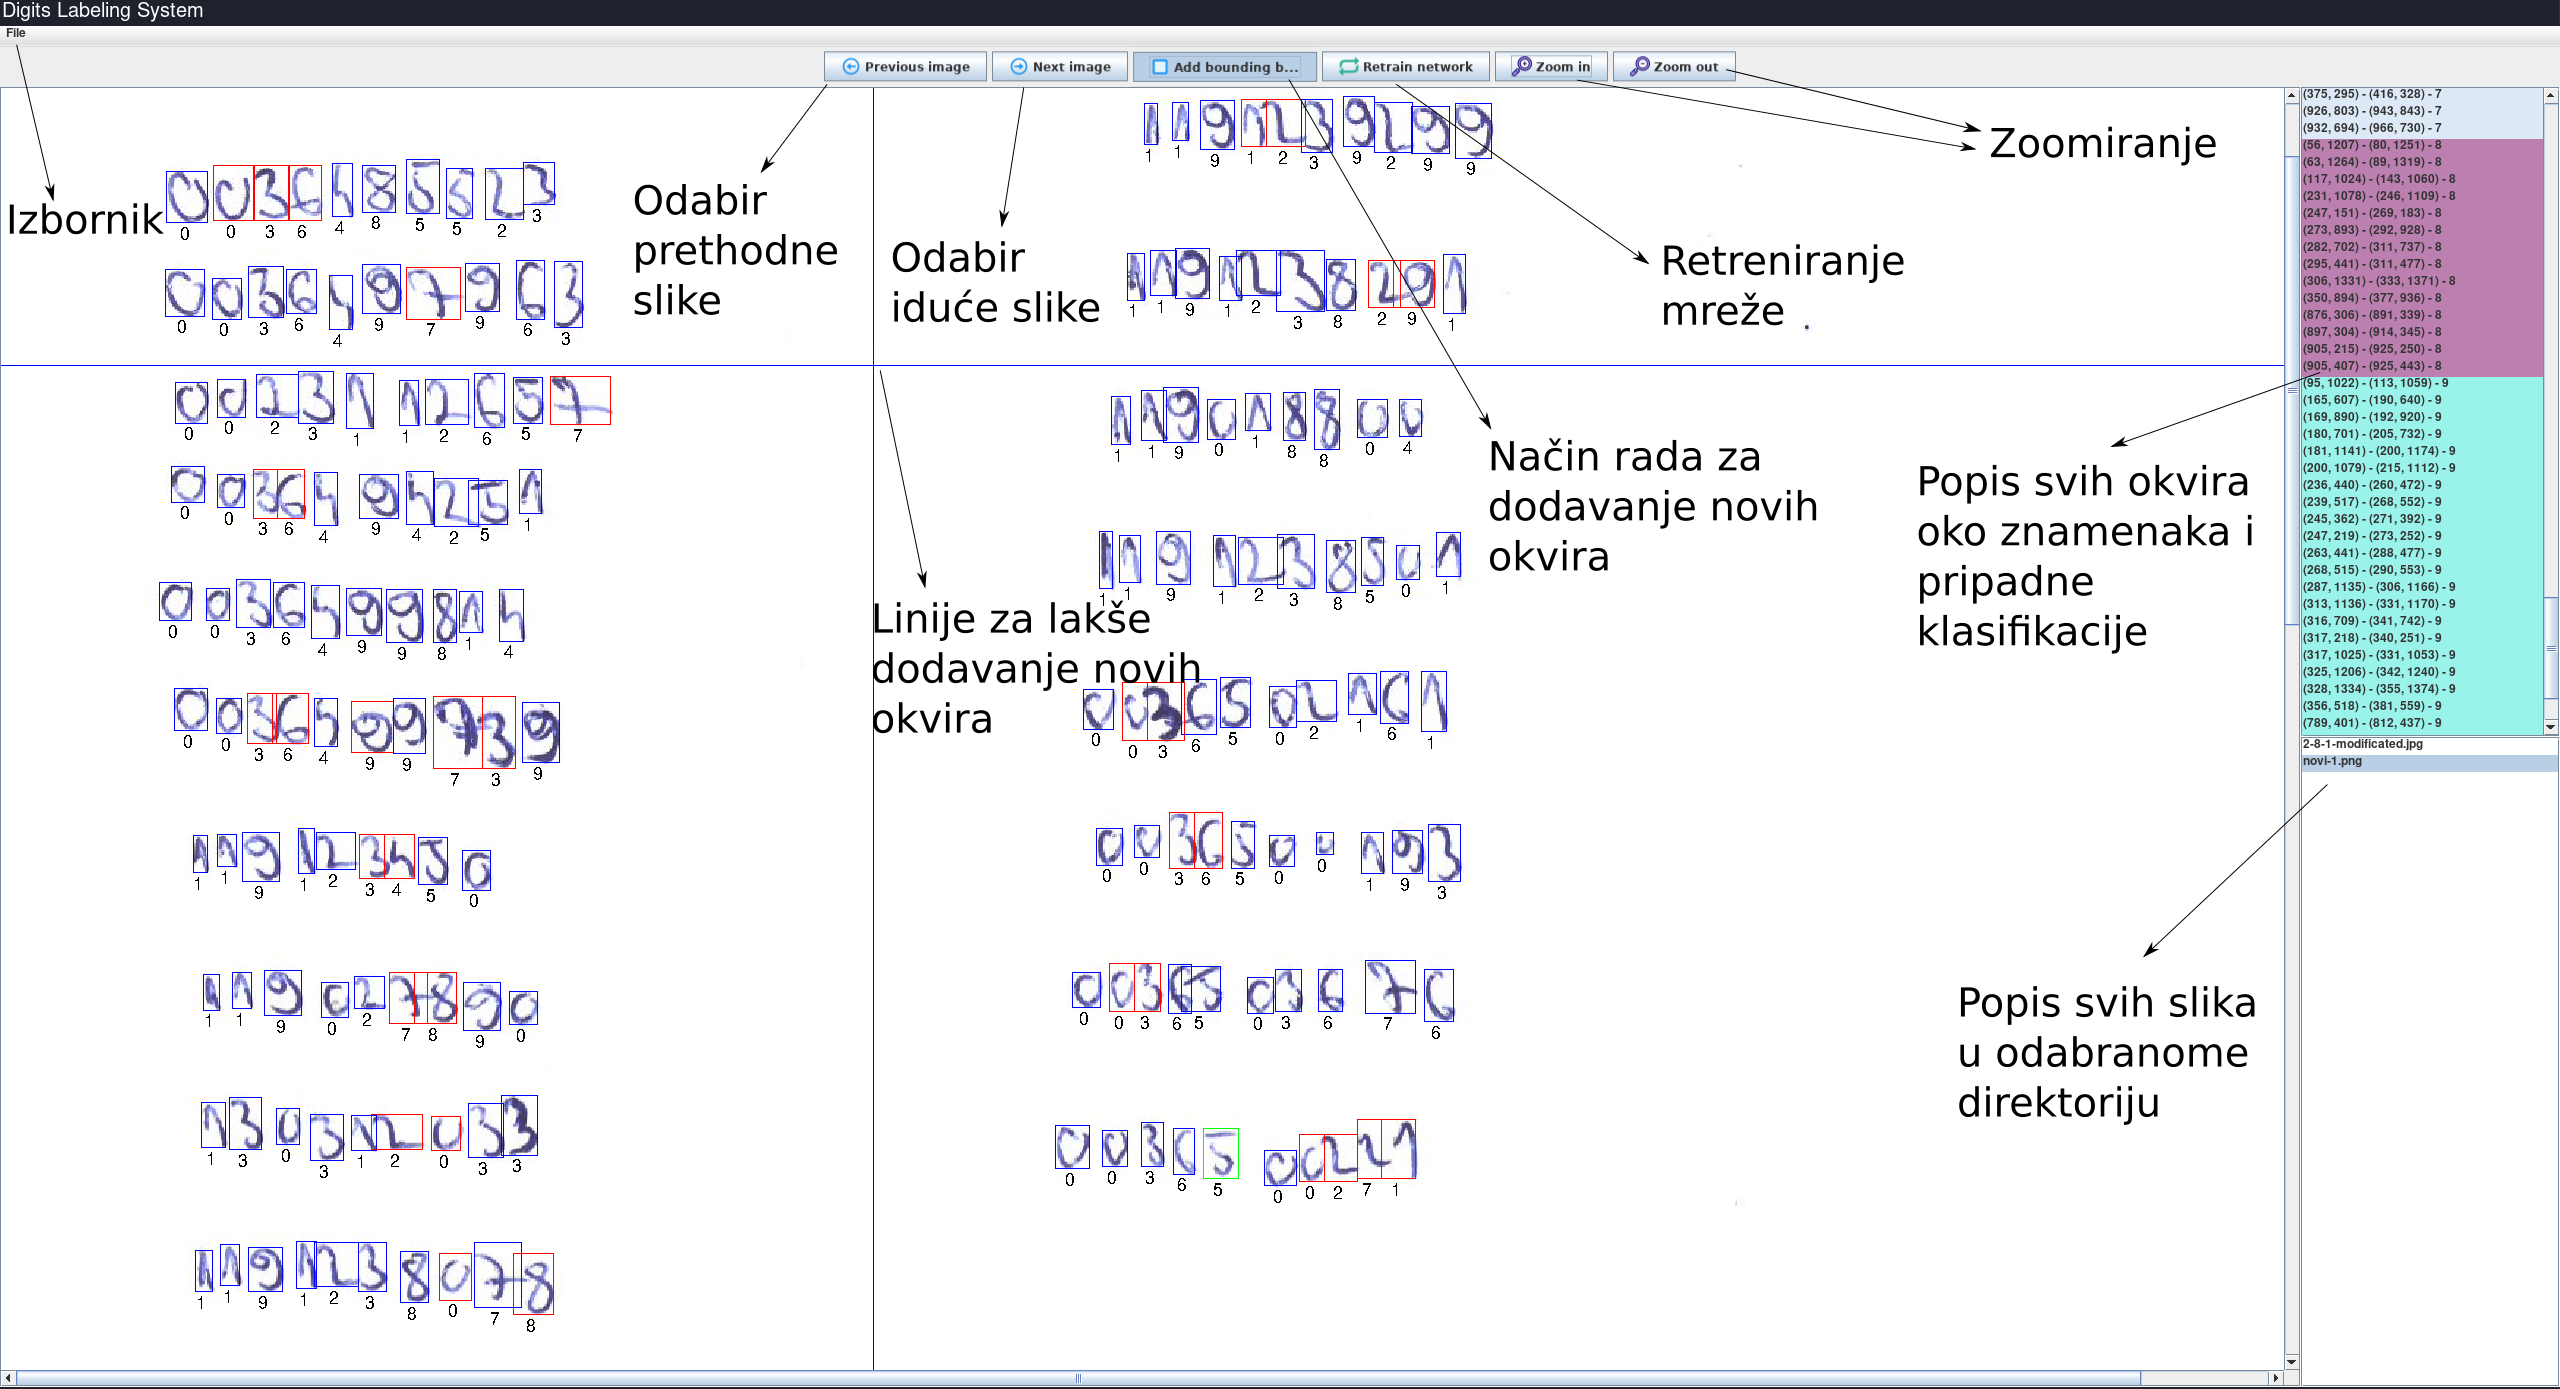
\includegraphics[scale=0.2]{master_detail.png}
\caption{Prikaz glavnog ekrana aplikacije}
\end{figure}



Nakon uspješnog labeliranja nudi se mogućnost retreniranja mreže s novo označenim znamenkama. Time se nudi mogućnost gradnje još većeg skupa za učenje, što u konačnici dovodi do robusnije klasifikacijske mreže. Također moguće je pohraniti odnosno učitati podatke o već prethodno labeliranim slikama. Radi boljih performansi svaki od graničnih okvira iscrtava se u zasebnom sloju iznad sloja u kojem se iscrtava slika kako ne bi bilo potrebe za ponovnim renderiranjem same slike. Dodatno, podatci o svakoj od označenih slika spremaju se u priručnu memoriju tijekom označavanja kako ne bi bilo potrebno čekati sustav da odradi lokalizaciju i klasifikaciju ako je već vidio odabranu sliku. Radi bolje preglednosti unutar popisa svih okvira oko znamenaka i pripadne klasifikacije sortirane su prvo po klasi [0-9], zatim po $x$ koordinati gornjeg lijevog ugla okvira te naposljetku po $y$ koordinati gornjeg lijevog ugla. Dodatno su pojedine klase vizualno separirane različitim bojama. \newline
Granični okviri koje pronađe algoritam temeljen na pronalasku spojenih komponenti odnosno kontura prolazi kroz dvije dodatne faze prije konačne odluke. U prvoj fazi predprocesiranja na temelju raznih filtera pokušavaju se eliminirati šumovi i spojiti okviri koji vjerojatno pripadaju istoj znamenci. Algoritam na temelju udaljenosti dvaju okvira pokušava razriješiti da li je potrebno spojiti okvire. Ako je udaljenost između okvira manja od najveće moguće definirane, promatra se omjer visina i širina. Dodatno se promatra dobiva li se spajanjem dvaju okvira novi okvir čija je visina odnosno širina znatno veća od prosječne visine odnosno širine. Eksperimentalnom metodom nad većim uzorkom izračunate su okvirni pragovi maksimalnog dozvoljenog omjera visina, širina i odstupanja od srednjih vrijednosti, te se na temelju ugrađenog znanja u sustav spajaju okviri koji vrlo vjerojatno čine jednu znamenku, no koje zbog kvalitete skeniranja ili loše otisnutog broja sustav nije prepoznao kao jednu spojenu konturu. Sustav rekurzivno spaja okvire, primjerice kaže li sustav da je potrebno spojiti okvir $B_1$ s okvirima $B_2, B_3$, te da je okvir $B_3$ potrebno spojiti s okvirima $B_4, B_5$, provodi se spajanje $B_1, B_2, B_3, B_4, B_5$ u jedan novi okvir. Sam sustav je testiran nad znamenkama pisanim različitim bojama kemijskih olovaka, tehničkim olovkama i običnim olovkama. Naposljetku sustav na temelju prosječne visine okvira eliminira šumove tako da traži one okvire koji su znatno manji od prosječne visine svih okvira. Ova faza je temeljena čisto na matematičkim pravilima koja opisuju \textit{a priori} znanje o tome kako čovjek piše znamenke. Primjerice očekivano jest da kada pišemo svoj identifikacijski broj da su nam znamenke približno iste visine, da pojedine znamenke odvajamo približno istim razmakom, da se držimo relativno linije pisanja odnosno da nam nije jedan broj gore na stranici a drugi na sredini stranice itd. Nakon završetka ove faze sustavu za klasifikaciju se prosljeđuju obrađeni okviri. Sustav na temelju njih vrši klasifikaciju i tako već klasificirane znamenke šalju se na postprocesiranje. \newline
U fazi postprocesiranja sustav može predvidjeti koje znamenke su vjerojatno krivo označene (primjerice sustav je spojio dva okvira u jedan, a unutra se nalaze dvije znamenke i slično). Po izlasku iz ove faze okviri i klasifikacije istih se prikazuju korisniku na grafičkom korisničkom sučelju. Oni okviri za koje pretpostavljamo da je sustav možda pogriješio, poprimaju crvenu boju, dok su preostali označeni plavom bojom. Prvi od postprocesora koji se koristi temelji se na izračunu prosječne širine okvira. Ako je širina okvira barem $1.5$ puta veća od prosječne širine, vjerojatno se radi o pogrešno označenoj znamenci. Drugi postprocesor se temelji na izlazu klasifikatora. Kako je izlaz klasifikatora diskretan probabilistički, odnosno kako je suma vjerojatnosti pojedinih klasa jednaka $1$, drugi postprocesor na temelju sigurnosti \engl{confidence} svoje odluke i zbunjenosti klasifikatora \engl{perplexity} pokušava pronaći krivo označene okvire. U teoriji informacija, zbunjenost je definirana kao mjera koliko dobro vjerojatnosna distribucija ili probabilistički model predviđa uzorak. Često se koristi za usporedbu probabilističkih modela. Što je mjera zbunjenosti manja, vjerojatnosna distribucija je bolja u predviđanju uzorka. Zbunjenost se matematički definira preko entropije \engl{entropy}, odnosno zbunjenost diskretne vjerojatnosne distribucije $p$ definiramo kao:

\begin{equation}
2^{H(p)} = 2 ^ {- \sum_{x}^{}p(x)\log_{2}p(x)},
\end{equation}
pri čemu je $H(P)$ entropija distribucije i $x$ pojedini događaj čiju vjerojatnost razmatramo. Općenito, entropiju možemo promatrati kao mjeru nesigurnosti ili neodređenosti tako da sama definicija zbunjenosti se pokazuje kao smislena. Maksimalna prihvatljiva zbunjenost modela dobivena je eksperimentalnim putem. Ako je sigurnost klasifikatora u svoju odluku manja od 50\% i ako je njegova zbunjenost veća od eksperimentalno dobivene vrijednosti, promatrani okvir se šalje na analizu kliznim prozorom \engl{sliding window}. Istovjetno se postupa ako je širina okvira barem $1.5$ puta veća od prosječne širine.
\newline
Metoda zadužena za analizu okvira kliznim prozorom pokušava koristeći različite veličine kliznog prozora razdijeliti okvir na dijelove kako bi zbunjenost modela bila minimalna. Metoda na početku za prvu od definiranih veličina kliznih prozora uzme prvih $N$ slikovnih elemenata okvira te računa zbunjenost modela. Zatim uzme još $N$ slikovnih elemenata okvira, dakle ukupno $2N$ slikovnih elemenata je širina okvira i ponovno računa zbunjenost modela. Analogno se okvir obrađuje dok se ne dođe do kraja slike. U tom trenutku računa se za koju širinu slike je postignuta najmanja zbunjenost. Ako je zbunjenost najmanja za inicijalni okvir, nastavlja se sa sljedećom veličinom kliznog prozora. U suprotnome, ulazni okvir se analizira ekvivalentno od točke za koju je utvrđeno da model ima najmanju zbunjenost. Dakle, nastavlja se analiza s preostalim dijelom okvira, a pronađeni okvir se dodaje u novi skup okvira. Nakon što završi analiza, traži se minimalna zbunjenost postignuta za različite veličine kliznog prozora. Kako bi se više kažnjavala veća zbunjenost prilikom traženja najadekvatnije podjele okvira računa se suma kvadrata zbunjenosti za svaku veličinu kliznog prozora. Dobivamo li primjerice za jednu veličinu prozora da je najmanja zbunjenost da se okvir uopće ne dijeli, dok za drugu veličinu prozora kao izlaz dobivamo da je najbolje okvir podijeliti na 3 dijela, potrebno je regulirati utjecaj pojedinih faktora u navedenoj sumi kako podjela sa samo jednim okvirom i relativno velikom zbunjenošću se ne bi preferirala naspram podjele koja daje znatno manje zbunjenosti, no u sumi dovodi do znatno većeg utjecaja. Konačan izraz korišten za traženje podjele s najmanjom zbunjenosti je dan u nastavku:
\begin{equation}
Utjecaj = \sum_{i = 0}^{i = broj\ okvira - 1} zbunjenost_{i}^2 \cdot  {\rm e}^{-i}
\end{equation}
Primjer u nastavku demonstrira rad sustava za predviđanje potencijalno pogrešno označenih okvira oko znamenaka. Izvorno su parovi znamenaka (3, 6), (9, 9) i (7, 3) imali po jedan granični okvir, odnosno bili su labelirani kao jedna znamenka. Sustav za postprocesiranje je na temelju prosječne širine, zbunjenosti i sigurnosti klasifikatora pretpostavio da se radi o pogrešci i ispravno označio okvire crvenom bojom. Metodom kliznog prozora sustav je uspješno razriješio situaciju i odvojio znamenke (3, 6) i (7, 3) i uspješno ih klasificirao, no znamenke (9, 9) ipak su ostale spojene u jedan okvir. Vidljivo je sa slike kako je donji završetak znamenke 9 spojen s gornjim dijelom, pa tako vjerojatno klasifikator nije uspio dobiti bolje rezultate koristeći metodu kliznog prozora zbog same nečitljivosti napisane znamenke. Pokazalo se da metodom postprocesiranja sustav gotovo uvijek ispravno pronađe "sumnjive" okvire, i u velikom broju situacija ih uspješno rješava. Označavanjem "sumnjivih" okvira crvenom bojom, korisnik odmah nakon uspješno odrađene lokalizacije i klasifikacije modela, ima vizualnu sugestiju okvira koje bi bilo poželjno ručno pregledati i eventualno napraviti izmjene. Nakon uvođenja podsustava za postprocesiranje, cjelokupni sustav je davao značajno kvalitetnije rezultate na "problematičnim" ulaznim slikama.
\begin{figure}[h]
	\centering
	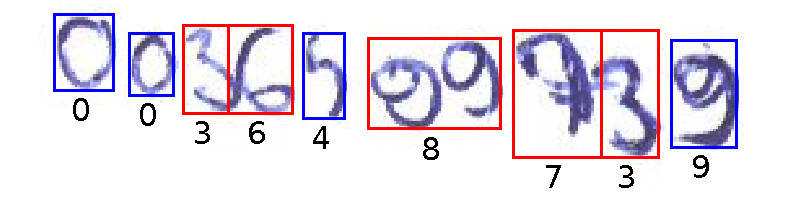
\includegraphics[scale=0.46]{postprocesor.png}
	\caption{Primjer rada podsustava za pronalaženje i razrješavanje sumnjivih okvira}
\end{figure}
\newline
Želi li korisnik promijeniti visinu/širinu okvira ili klasifikacijski broj, dvoklikom na željeni okvir na slici ili unutar popisa svih okvira otvara se dijalog s mogućnošću izmjene. Odmah prilikom izmjenjivanja vrijednosti na grafičkom korisničkom sučelju prikazuju se promjene. Naravno, u bilo kojem trenutku moguće je odustati od izmjena ili potvrditi napravljene izmjene. Prilikom prelaska mišem preko slike, kada se pokaznik nalazi iznad pojedinog okvira on biva "prekriven" transparentnom ljubičastom bojom radi lakše vizualizacije u situacijama kada slika sadrži gusto napisane brojeve gdje se njihovi granični okviri preklapaju.
\begin{figure}[h]
	\centering
	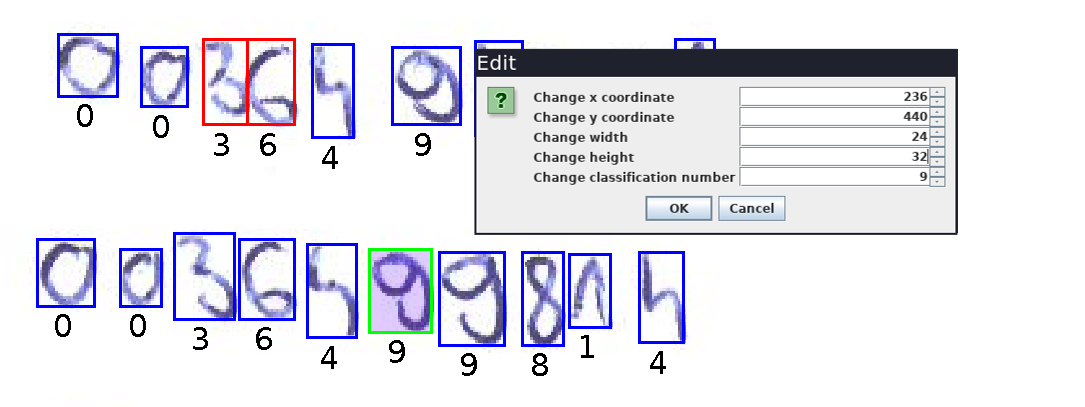
\includegraphics[scale=0.5]{edit.png}
	\caption{Uređivanje postojećeg graničnog okvira}
\end{figure}
Prilikom pohrane označenih slika za svaku od labeliranih slika pohranjuje se putanja do slike, koordinate gornjeg lijevog ugla svakog okvira oko znamenke, širina, visina okvira i klasifikacijski broj. Analogno, samo u suprotnome smjeru, vrijedi za učitavanje pohranjenih podataka. Ako se u odabranome direktoriju već nalazi slika za koju smo učitali podatke iz prethodno pohranjenog skupa podataka, sustav prilikom odabira iste slike ne vrši lokalizaciju i klasifikaciju znamenaka već automatski učita podatke o pozicijama i klasifikacijama iz učitanog skupa podataka kao što je ranije spomenuto.
\newline
Prilikom označavanja svake od slika, u svrhu generiranja preciznog i konzistentnog skupa podataka moguće je vršiti uvećavanje odnosno umanjivanje slike s faktorom $1.1$.
\newline
\newline
\begin{figure}[h]
	\centering
	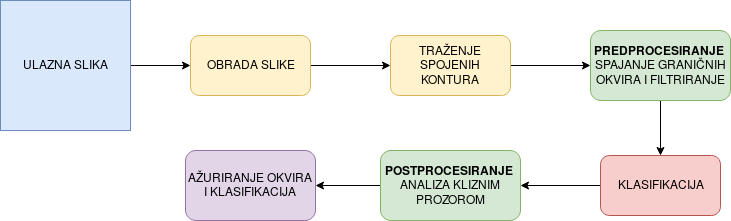
\includegraphics[scale=0.6]{system_arhitecture.png}
	\caption{Tok obrade ulazne slike kroz izgrađeni sustav}
\end{figure}



\chapter{Rezultati}
Izgrađeni sustav je pokazao na sakupljenom skupu od nešto više od desetak različitih distribucija sakupljenih rukopisa vrlo dobre rezultate. Na ulaznim uzorcima na kojima su znamenke bile razmaknute, sustav je u velikom postotku uspješno pronalazio granične okvire i klasificirao iste. Nakon izrade postprocesora, značajan napredak se pokazao i na slikama gdje su znamenke vrlo gusto napisane.
Prilikom implementacije isprobano je više različitih metoda procesiranja ulazne slike i klasifikatora. Prilikom procesiranja ulazne slike, pokazalo se da stanjivanje kontura \textit{Zhang-Seunovom} metodom ne doprinosi značajnijim rezultatima u radu klasifikatora. Zbog toga prilikom obrade ulazne slike kao što je ranije spomenuto, dilatacija je zadnji korak pri obradi slike. Također, isprobano je više različitih modela s različitim brojem slojeva, aktivacijskim funkcijama, različitim skupovima za učenje i ispitivanje. Model učen samo na MNIST skupu za učenje je postigao bolje rezultate prilikom evaluacije modela na testnome skupu iz istog MNIST skupa podataka, no na stvarnim uzorcima su rezultati bili mnogo lošiji od rezultata dobivenih nad vlastitim skupom za učenje i testiranje. Uz izgrađeni sustav za lokalizaciju i klasifikaciju promatrani su duboki modeli specifični za detekciju objekata na slici. Neki od najpoznatijih takvih modela su konvolucijske neuronske mreže temeljene na regijama (\textit{R-CNN, Fast R-CNN, Faster R-CNN,  ...}) čije već istrenirane modele nad poznatim skupovima podataka možemo pronaći u  aplikacijskom programskom sučelju \textit{TensorFlow Object Detection}. Isproban je jednostavan primjer koristeći  model \textit{You only look once} (YOLO) za detekciju objekata, no zaključeno je na testnome problemu da će kvalitetnije svoju zadaću obavljati sustav implementiran u ovome radu. U konačnici, implementirani sustav s visokim postotkom uspješnosti rješava lokalizacijske i klasifikacijske probleme rukom pisanih znamenaka odnosno identifikatora.

\chapter{Zaključak}
Cjelokupan rad se pokazao vrlo zanimljivim. Povezao je područja iz obrade slike, dubokog učenja, teorije informacija, arhitekture sustava, optimizacije i izrade aplikacija s grafičkim korisničkim sučeljem. Kako je svaki od podsustava implementiran samostalno, izradom rada dobio se uvid u mnoge aspekte iz raznih područja. Implementacijom metoda koje se svakodnevno koriste u biblioteci \textit{OpenCV} za obradu slika, osmišljanjem i implementacijom metoda za predprocesiranje i postprocesiranje pronađenih graničnih okvira, osmišljanjem arhitekture cjelokupnog sustava a zatim i optimizacijom dodano je znanstveno-istraživačko ruho radu. Mješavinom zaključaka stečenih učenjem klasifikatora i matematičkim pretpostavkama o problemu dobiveni sustav se vrlo dobro nosio s problemima lokalizacije i klasifikacije.
Potencijalna unaprjeđenja možemo usmjeriti ka sustavu za postprocesiranje graničnih okvira, odnosno podsustavu zaduženom za pronalazak pogrešno označenih graničnih okvira.  Povećanjem skupa za učenje uzorcima različitih autora, sustav za klasifikaciju bi postao robusniji i bolje se nosio sa specifičnim rukopisima. Samim time podsustav koji na temelju entropije i zbunjenosti klasifikatora razrješava potencijalno krivo označene okvire  bi se kvalitetnije nosio s navedenim problemom. Eksperimentiranjem nad matematički modeliranim znanjem koristeći različite distribucije rukopisa  možemo fino ugađati model i pokušati pronaći optimalne parametre.  Samo uvođenje sustava za postprocesiranje sumnjivih graničnih okvira  značajno je poboljšalo rad cjelokupnog sustava, te je potreba za ručnom intervencijom korisnika svedena na nisku razinu. 

Izradom ovog rada stečen je uvid  o algoritmima koji se koriste u poznatim bibliotekama, odnosno kako pojedini algoritmi rade "ispod haube". Istraživački dio približio je probleme s kojima se susreću autori novih algoritama odnosno metoda za obradu slika.
\nocite{*}

\bibliographystyle{fer}
\bibliography{literatura}

\begin{sazetak}
	Prepoznavanje rukom pisanih znamenaka popularno je od samih ambicioznih početaka strojnog i dubokog učenja. Ovaj rad opisuje sustav koji osim prepoznavanja vrši i lokalizaciju, odnosno vrši detekciju pojedine rukom pisane znamenke. Sustav na ulazu prima sliku rukom pisanih identifikatora koja transformira u binarnu i vrši se podebljanje kontura. Na temelju visine, širine i odnosa između graničnih okvira vrši se spajanje i filtriranje pronađenih komponenti. U fazi postprocesiranja na temelju širine okvira te sigurnosti i entropije klasifikatora pronalaze se problematični granični okviri i metodom kliznog prozora pokušavaju se razriješiti isti. Analiza se vrši koristeći dinamičku veličinu prozora te se na temelju zbunjenosti modela vrši podjela. Sustav je ukomponiran u aplikaciju s jednostavnim i intuitivnim grafičkim korisničkim sučeljem. Problematični granični okviri vizualno se ističu kako bi korisnik lakše uočio i ispravio eventualne pogreške sustava. Omogućeno je uređivanje pronađenih graničnih okvira i pripadnih klasifikacija. Sustav tako omogućava generiranje sve većeg skupa za učenje i ponovno treniranje mreže na novoizgrađenom skupu rukom pisanih identifikatora čime klasifikator postaje  još robusniji. 
	
	\kljucnerijeci{duboki modeli, konvolucijske neuronske mreže, obrada slike, lokalizacija, klasifikacija, rukom pisani identifikatori, povezane komponente, entropija, metoda kliznog prozora.}
\end{sazetak}
\newpage
% TODO: Navedite naslov na engleskom jeziku.
\engtitle{Deep Models Based Recognition of Student Identifiers}
\begin{abstract}
	  Recognition of handwritten digits is popular from the ambitious beginnings of machine and deep learning. 
	  This paper describes a system that  apart from recognizing, also performs localization, or performs detection of  handwritten digits. The system at the entrance receives an image of handwritten identifiers that is transformed into binary 
	  and contours of the identifiers are bolted.  Based on the height, width and relationship between the boundary boxes, merging  and filtering of the found boxes are performed. In the postprocessing phase based on the width of the box, classifier's confidence and perplexity (entropy), problematic boundary boxes are found and the sliding window method is applied to resolve these boxes. The analysis is done using the dynamic size of the sliding window and based on the perplexity of the model  the division of the boundary box is performed. The system is wrapped in an application with a simple and intuitive graphical user interface. The problematic bounding  boxes are visually highlighted so that the user can easily detect and resolve possible system errors. Through the graphical interface it is possible to edit the found boundaries and the corresponding classifications. The system thus enables the generation of ever larger learning dataset and retraining the network on a newly built dataset of handwritten identifiers that make the classifier even more robust.
	  
\keywords{deep models, convolutional neural networks, image processing, localization, classification, handwritten identifiers, connected components, entropy, perplexity, sliding window.}
\end{abstract}

\end{document}
